% !TeX root = ./article.tex
\documentclass[manuscript,linenumbers]{aastex63}

\usepackage{xspace}

\newcommand{\ang}[1]{#1\degr}
\newcommand{\eg}{\textit{e.g.}\xspace}
\newcommand{\ie}{\textit{i.e.}\xspace}
\newcommand{\change}[1]{{\color{cyan}#1}}

\received{January 30, 2020}
\revised{October 6, 2020}
\accepted{October 21, 2020}
\published{January 25, 2021}
\submitjournal{AstroPhysical Journal}

\shorttitle{Titan's haze seasonal variations}
\shortauthors{Seignovert et al.}

\begin{document}
\title{Haze seasonal variations of Titan's upper atmosphere\\during the Cassini Mission}

\author[URCA,JPL]{Beno\^{i}t Seignovert\corref{correspondingauthor}}\ead{research@seignovert.fr}
\author[URCA]{Pascal Rannou}
\author[JPL]{Robert A. West}
\author[LESIA]{Sandrine Vinatier}

\address[URCA]{GSMA, Universit\'{e} de Reims Champagne-Ardenne, UMR 7331-GSMA, 51687 Reims, France}
\address[JPL]{Jet Propulsion Laboratory, California Institute of Technology, Pasadena, CA 91109, USA}
\address[LESIA]{LESIA, Observatoire de Paris, Universit\'{e} PSL, CNRS, Sorbonne Université, Université de Paris, 5 place Jules Janssen, 92195 Meudon, France}

\cortext[correspondingauthor]{Corresponding author}

The 13 years of the Cassini mission provide a unique dataset monitoring
the evolution of Titan’s atmosphere during almost half a Titan's year,
between the middle of the northern winter up to the northern summer solstice.
In this work we present a survey of the haze vertical extinction profiles retrieved
between 300 to 700 km with an atmospheric limb multiple scattering model.
We analyze 138 ISS NAC CL1-UV3 images taken between 2004 to 2017 covering the
entire Cassini mission.
We mainly focus our attention on the temporal evolution of the haze content
in the upper atmosphere to track the evolution of the detached haze layer.
As previously reported by \cite{West2011}, the detached haze layer is present
at all the latitude below \ang{60}N and collapse globally on the main haze
before the vernal equinox in 2009.
No permanent detached haze layer is observed between 2012 and 2015 but
we show that at the end of 2015, a new structure emerges from
the summer hemisphere (north) and propagate to the equator. This new layer
is not as pronounced and is much more complex than the one observed at the
beginning of the mission but is likely to be the initiation of a new detached haze layer.
We also investigate the short time scale variability of the detached haze
layer and no major changes is observed. Finally, we report some cases
where the viewing geometry allows us to probe the longitudinal variability
of the haze, highlighting some local inhomogeneities.
All these observations bring new perspectives
on the seasonal cycle of Titan's upper atmosphere, the evolution of the detached
haze layer and its interaction with the dynamics.
The main seasonal pattern predicted by the global circulation models is consistent
with our findings, but the details and the timing of the global collapse
is not yet explained. Finally, comparisons with the UVIS instrument shows
that the haze extinction profiles retrieved during two stellar occultations
in 2009 are consistent with our results.
\section{Introduction}

Titan is the only moon of the solar system with a thick hazy atmosphere which represents approximately 20\% of its apparent
diameter. This atmosphere is mainly composed of nitrogen and methane. The photo-dissociation of these molecules by the
UV light in the upper part of the atmosphere leads to the production of a large number of other hydrocarbons and nitriles as
trace species and to photochemical haze. This haze is global and completely covers Titan. It controls
the thermal balance through its visible and thermal infrared properties \citep[e.g.][]{Bezard2018}.
It also veils the lower atmosphere and the surface that can be perceived in a few methane windows in near infrared.

Titan's haze was first resolved in the 80's by Pioneer 11 \citep{Smith1980} and the two Voyagers
\citep{Smith1981, Smith1982, Sromovsky1981}. It had several remarkable structures: a northern (winter)
polar hood, an interhemispheric asymmetry and a thin global detached haze layer (DHL) above the main global haze layer. It was
thought that the detached haze layer had a dynamical origin \citep{Smith1981}. Photometric analyses provided a means
to derive the extinction properties of both haze layers and to evaluate the effective radius of the aerosols in the detached
haze ($\simeq 0.3 \mu$m) and in the main haze ($\simeq 0.4 \mu$m) layers \citep{Rages1983, Rages1983a}. Analysis of Voyager images showed
that the detached haze layer appears due to a strong depletion of aerosol extinction around 300 km, yielding a distinct
layer above the main haze layer with a maximum extinction located around 350 km \citep{Rages1983}. Its horizontal extent was
very stable in pressure and it was reported at all the southern latitudes up to \ang{45}N where it connected to the northern
polar hood. The detached haze layer was re-observed twenty years after the Voyager flybys during Cassini first flyby in 2004
\citep{Porco2005}. The main change was in its altitude location at 500 km, which was 150 km higher than in 1981.
Again, it appeared as a fairly homogeneous global shell above the main haze layer at a constant altitude and
merged with the northern polarhood. Notably, while Voyager observations were performed after the northern spring equinox,
Cassini early observations occurred during the northern winter, that is half a season earlier (Fig.~\ref{fig:titan_seasons}).

\begin{figure}[!ht]
    \centering
    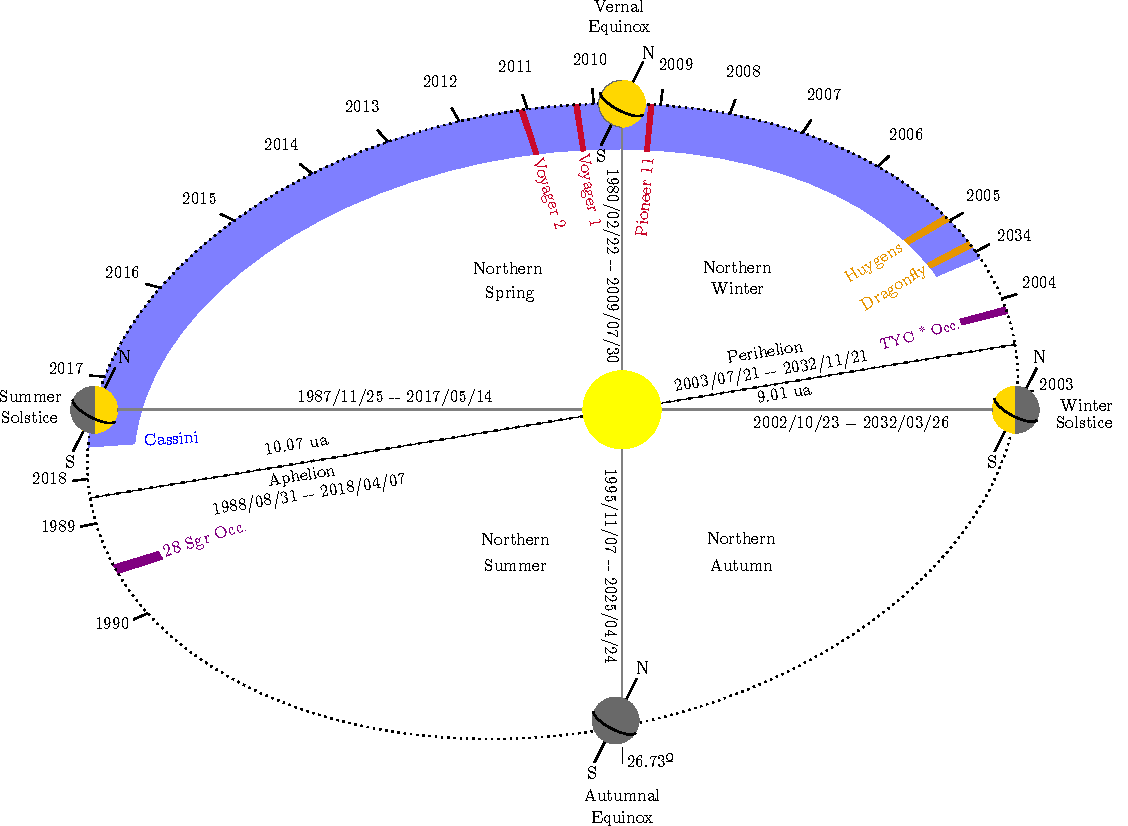
\includegraphics[width=\textwidth]{Fig/Titan_seasons}
    \caption{Titan orbital position as a function of the season, reported as solar longitude position ($L_s$).
             The Cassini mission covered almost half a Titan year. The Pioneer and Voyager flybys are also reported
             as well as the Huygens landing and ground-based stellar occultations observed on Earth.}
    \label{fig:titan_seasons}
\end{figure}

 \cite{Toon1992} first attempted to explain the observation of the DHL. They used a 1D microphysical
model where an \emph{ad hoc} vertical wind maintains aloft the DHL particles at a constant altitude above the main
haze layer. Alternative scenarios were proposed to explain the DHL from purely microphysical processes. \cite{Chassefiere1995}
investigated the case of two different aerosol production layers. They proposed that the uppermost layer (500-1000 km)
produces fluffy aggregates that could be swept horizontally by winds, generating a detached haze layer. They also
proposed an alternative scenario where aerosols settle downward and interact with macromolecules from the main haze layer,
produced by the lower production zone (around 350-400 km). In the latter case, the interaction would produce by some
way an optical gap. However, they favored the scenario involving winds which would match all the constraints
known at that time. In the same vein, \cite{Lavvas2009} proposed a scenario based on a purely microphysical process. Aerosols
are produced at high altitude, as per the \cite{Chassefiere1995} hypothesis, growing as spheres down to levels around 500 km.
But there, the detached haze is produced by a sudden change in the fractal dimension of the aerosols. This produces a
sharp change in the microphysical properties, and an artificial optical gap. However, it is unclear how this model for the
production of the detached haze layer would be augmented to account for the seasonal evolution of the altitude,
disappearance, and reappearance (as described below).

Later, with a 2D-General Climate Model (GCM) accounting for the transport of haze by dynamics and the radiative
feedback, it was possible to reproduce and explain the mechanism that produces the DHL \citep{Rannou2002}. It was also
demonstrated that this feedback strongly enhances the wind speed due to the thick polar haze cap near the winter pole.
In return, this cap enhances the cooling to space during the polar night \citep{Rannou2004} and
reinforces the circulation. Due to Titan's obliquity (\ang{27}) and the slow rotation rate, seasons are well
marked and Hadley circulation cells span both hemispheres. This situation leads to the formation of a
broad ascending circulation in the summer hemisphere able to lift aerosols up to high altitudes where they remain
suspended and are transported through mid-latitudes to the winter polar region where they are transported by
subsidence (Fig.~\ref{fig:titan_atm_circulation}). In this scenario, the location of the DHL corresponds to the area
where the settling speed is compensated by upward wind and evolves with seasonal changes of illumination.
More sophisticated 3D-GCMs improved the understanding of the haze cycle, including the formation of the detached haze,
and confirmed this picture \citep{Lebonnois2012,Larson2015}. This formation mechanism implies that the DHL
is a blending of aerosols newly produced and falling from above and older and larger aerosols produced in the
stratosphere and lifted by circulation.
Although the GCM results differ in some aspects with observations, they are able to capture the main picture behind
the existence of the DHL.

\begin{figure}[!ht]
    \centering
    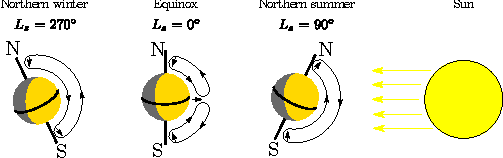
\includegraphics[width=.47\textwidth]{Fig/Atmsopheric_circulation}
    \caption{Synthetic representation of Titan atmospheric circulation as a function of season.}
    \label{fig:titan_atm_circulation}
\end{figure}

Photometric studies performed with Cassini data taken before the equinox in 2009 provide complementary observations
of the DHL \citep{Cours2011, Koskinen2011, Seignovert2017}.
On one hand, the authors used the light intensity scattered at the limb in UV (338 nm)
at different phase angles measured by ISS. On the other hand, a single value of the tangential opacity in VUV (187 nm)
was retrieved from UVIS observations during stellar occultations.
The results show the presence of large aerosols in the DHL with an effective bulk radius $\simeq 0.2\ \mu$m,
producing all the UV scattering, while small nanometric aerosols are needed to explain most of the VUV
extinction \citep{Cours2011}, which is quite consistent with a DHL made of two different populations of
aerosols.

\cite{West2011} also reported a rapid collapse of the detached haze layer starting just before the equinox. The altitude of
the DHL descended by about 80 km in 200 terrestrial days and by 30 km more in about 300 terrestrial days. A simple
extrapolation of the altitude of the DHL with time indicated that it would be at the same altitude as observed by Voyager
exactly one Titan year after the Voyager epoch. \cite{West2011} concluded that such a result was coherent with a seasonal
cycle of the DHL.  They compared their results with a 2D-GCM \citep{Rannou2002} and made a prediction about the reappearance of the
DHL several years later (2013-2016) at its initial altitude (around 500 km). \cite{Lebonnois2012} and \cite{Larson2015} made
similar predictions but with a reappearance of the DHL a bit later, around the next northern summer solstice ($L_S=\ang{95}$
and $\ang{70}-\ang{80}$, respectively). In practice, \cite{West2018} found that the DHL reappeared in early 2016
($L_S=\ang{73}-\ang{76}$) at 480 km, several months before the solstice (mid-2017). They followed the cycle of the DHL at the equator
and retrieved the haze extinction profile in the CL1-UV3 filter combination.
Its reappearance was much more complex than predicted. This early 2016 detached haze layer
dropped in altitude down to 470 km within a terrestrial year and vanished while a new DHL emerged again around 500 km. This
new layer appeared quite stable until the end of the Cassini mission (September 2017, $L_S=\ang{91}$). Unfortunately, no other
data exist to further probe the DHL and nothing is known about the fate of the detached haze after this date.

\medskip

In the present work, we perform a systematic latitude-altitude mapping of the detached haze layer in the range 350 to 600 km altitude.
This covers the period between July 2004 (half a season after the northern winter solstice) and the end of
the mission in September 2017 (after the summer solstice).
We used all the UV3 observations acquired by the Cassini Narrow Angle Camera (NAC) of ISS.
We used exactly the same model as \cite{West2018}, that is a ray tracing model in spherical shell geometry for the single-scattering albedo
and a correction for multiples scattering.

The outline of the article is as follows. In the next section (\textbf{section 2}), we first give a global presentation of
the available data and the criteria we use to select images.
Then we describe the main principle of the retrieval model and the retrieval method.
In \textbf{section 3} we present the results of the photometric analysis as latitude -
altitude panels showing the spatial distribution of the DHL and the upper part of the main haze layer.
The seasonal cycle of the DHL is split in four specific periods between 2004 and 2017.
This section has then 4 subsections for each period where we explain in detail the main characteristics of the haze and
its evolution.
\textbf{Section 4} is dedicated to the study of specific sets of observations that probe short time scales,
short term or diurnal variations. We first describe how the data were selected and then what they reveal about Titan's atmosphere.
In \textbf{section 5}, we make comparisons between our results and results obtained at the same location and the same time with UVIS.
We also make comparisons between our results and prediction made by two Titan 3D-GCMs about the detached haze layer and its evolution.
The conclusion and the perspective of this work are given in \textbf{section 6}.

\section{Observations and models}

\subsection{Selection of observations}
We conduct our survey on 138 images\footnote{The list of all the ISS images analyzed is provided in supplementary.} taken by the Cassini Image Science Sub-System Narrow Angle Camera (ISS-NAC) with the
clear and ultra-violet filter combination CL1-UV3. At this wavelength (338 nm), ISS is sensitive to haze in the
upper part of Titan's atmosphere (300-600 km altitude). We choose the best sample among the 317 images available on the NASA Planetary Data System (PDS)
to get the highest temporal and phase coverage. For the main study we kept only images taken with at least a one-day gap.
We also kept specific sets of observations made a few hours apart to study short-term variations.

On average, the selected images are separated by 39 Earth days, \textit{i.e.} 2.5 Titan days (Fig.~\ref{fig:img_sampling}).
Although our sampling is not evenly distributed, due to orbital constraints and mission schedule, at least 90\% of the selected
images are separated by less than 120 Earth days, \textit{i.e.} 7.5 Titan days. Two main gaps of data can be observed.
The first is between 28 March 2008 and 25 January 2009 (302 Earth days) and 26 November 2010 and 9 September 2011 (286 Earth days).

\begin{figure}[!ht]
    \centering
    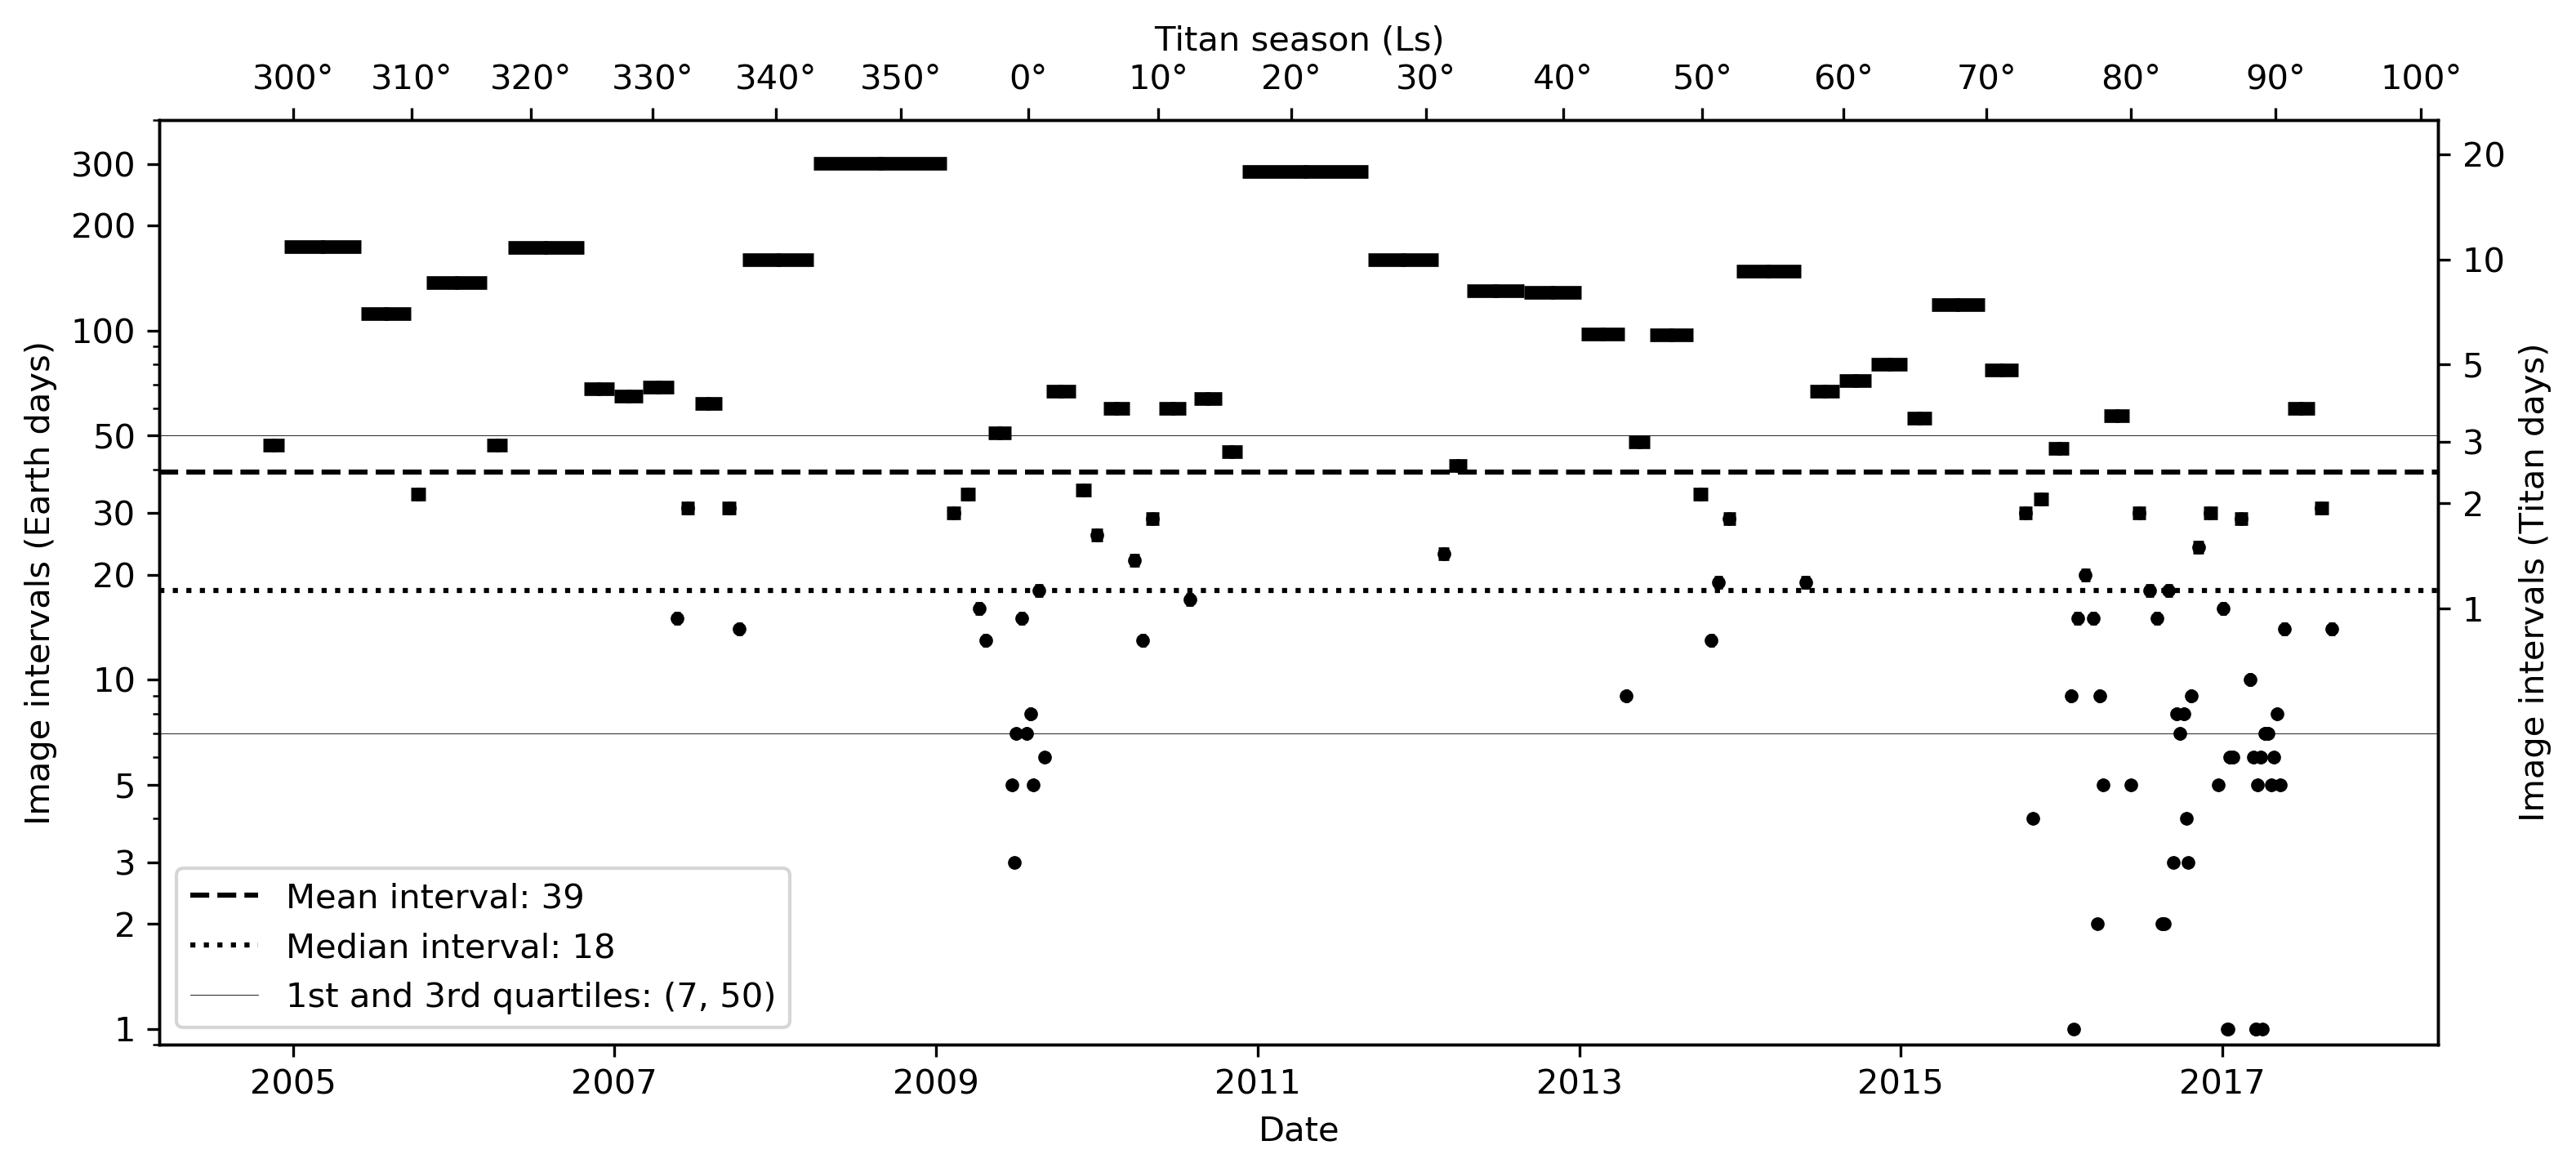
\includegraphics[width=\textwidth]{Fig/IMG_interval.png}
    \caption{Image intervals (in Earth and Titan days) between consecutive ISS/NAC CL1-UV3 observations analyzed.
        The length of the lines correspond to the duration between two acquisitions.}
    \label{fig:img_sampling}
\end{figure}

The selected images are calibrated using the CISSCAL routines (v3.8) provided on the Planetary Data System. To improve
the signal to noise ratio on the limb profile, we deconvolved the images with a Poisson Maximum a posteriori method
(PMAP) using the point spread function (PSF) measured in-flight \citep{West2010}. The image pointing is
initialized with the SPICE kernels \citep{Acton1996, Annex2017}. Since the surface of Titan is not visible in the UV, we improved
the location of Titan's center by fitting the limb intensity. Then, we calculated the planetocentric coordinates of each
pixel and their tangent point altitude with respect to a mean spherical body with a radius of 2575 km.

Intensity profiles are extracted every \ang{5} on both sides of the limb. Depending on the
latitude of the Sub-Cassini point on the ground, the sampling in latitude is not evenly distributed for each image.
Therefore, the polar latitudes are usually less covered than the equator.
Also, the solar illumination changes drastically during the
season between the northern mid-winter to summer, which restricts our ability to see both poles at the same time.


\subsection{Model of scattering at the limb}

To retrieve the haze extinction profiles from the intensity observations, we model the synthetic
radiance factor ($I/F$) with a single scattering ray tracing model in a spherical shell geometry.
The effect of multiple scattering is accounted for as a correction  $\varrho_k\left(z\right)$
applied to the volume scattering along line of sight.
This technique was used successfully several times before \citep[e.g.][]{Rages1983, Rannou1997, Seignovert2017, West2018}.

In the detached haze layer, the multiple scattering is mainly produced by the light coming from the atmosphere below. To
evaluate $\varrho_k$, the scattering properties of the atmosphere are fixed to
reproduce the observed intensity of Titan in the UV. With a radiative transfer model \citep[SHDOMPP, from ][]{Evans1998}
we have access to the complete radiative source function at each level of the atmosphere. We are then able to compare the
intensity that is scattered in the direction of the observer from the direct sun only and from the direct sun and the scattered
field coming from below. $\varrho_k$ is defined as the ratio of multiple scattering to single scattering toward the observer
for a given altitude and as a function of the incident and emergent angles. This parameter is pre-computed as a function of
altitude, incident and emergent angles and saved in a look-up table \citep[see.][for details]{West2018}.
We find that the multiple scattering increases the scattered intensity at the limb of Titan in the UV by a ratio between
1.05 and 1.15, depending on the geometry of the observation.

We discretize the atmosphere in $N=60$ irregular layers of various thickness : $\Delta z =$ 50 km from the
ground to 200 km, $\Delta z =$ 25 km from 200 to 300 km, $\Delta z =$ 10 km from 300 to 400 km and from 550 to 700 km.
Finally, we used $\Delta z$= 5 km between 400 and 550 km. This grid allows us to take advantage of the spatial resolution
of the ISS NAC camera in the region of interest where is mainly located the DHL.

We can write the outgoing $I/F (z)$ as:

\begin{equation}
I/F (z) = \sum_{i=0}^{n_x-1} \int\limits_{x_k}^{x_{k+1}}
\frac{\left< \varpi P(\Theta) \right>_k}{4}
e^{-\left( \tau^i_k\left(z\right) + \tau^e_k\left(z\right) \right)}
\beta_k\left(z\right) \varrho_k\left(z\right) d{x}
\label{eq:west2017_sup_limb}
\end{equation}

where the summation is performed on the $n_x-1$ segments defined by the intersections of the line of sight and the
spherical shell boundaries. The impact parameter $z$ (the lowest altitude reached by the line of sight) is given by the
bottom of the $n^\mathrm{th}$ layer crossed. Therefore, each layer of the atmosphere is crossed twice. $x$ is the
abscissa along the line of sight. $\tau^i_k$ and $\tau^e_k$ are the opacities along the incident and emergent paths.
$\left< \varpi P(\Theta)\right>_k$ is the average of the product of the single scattering and the phase function
at the scattering angle of the observation $\Theta$ for the layer crossed on $x_k$.  $\beta_k(z)$ is the local
extinction at altitude $z$. Here, the altitude $z(x)$ is the local altitude at point of abscissa $x$ along the
line of sight.


\subsection{Retrieval method}

Based on our previous work \citep{Seignovert2017, West2018}, we make the assumption that the optical properties
$\left<\varpi P(\Theta)\right>_k$ of the aerosols are constant in the upper part of Titan's atmosphere. This allows
us to focus our study only on the retrieval of the extinction along the line of sight.
In our model, the $I/F (z)$ intensity profiles depend on the set haze extinction profile $\beta(z)$ and the viewing
geometry of the observation (incidence, emergence and phase angles).
We assume no horizontal in-homogeneity along the line of sight \citep{Seignovert2017}. We retrieve a set of extinction values $\beta_i$ (
the vector ${\beta}$), with $i$ the indices of the layers, that matches the values of the $I/F_i$
(the vector $I/F$).

From the Eq. (\ref{eq:west2017_sup_limb}), it is possible to cast the scattered intensity $I/F_i$, as a function of
the extinction $\beta_j$ with $j \le i$. This forms a non-linear triangular system. To find the vector $\beta$, we
have to solve the formal equation:

\begin{equation}
    I/F = G(\beta)
\end{equation}

where ${G}$ is a nonlinear function which depends on $\beta_i$ and on the viewing geometry of the observation.

We solve the system by minimizing globally the difference between the modeled $I/F$ and the observations
using a Levenberg-Marquardt minimization. Therefore, we obtain simultaneously all the $\beta_i$ at once.
Moreover, the tangential opacity along a line of sight ($\tau_{los}$) is considered opaque when it reaches 3.
Beyond this threshold, we do not retrieve the value of $\beta$.
An example of inversion is presented in the figure~\ref{fig:model_uncertainties}.

\begin{figure}[!ht]
    \centering
    \includegraphics[height=6.5cm]{Fig/N1551888681_sampling.png}
    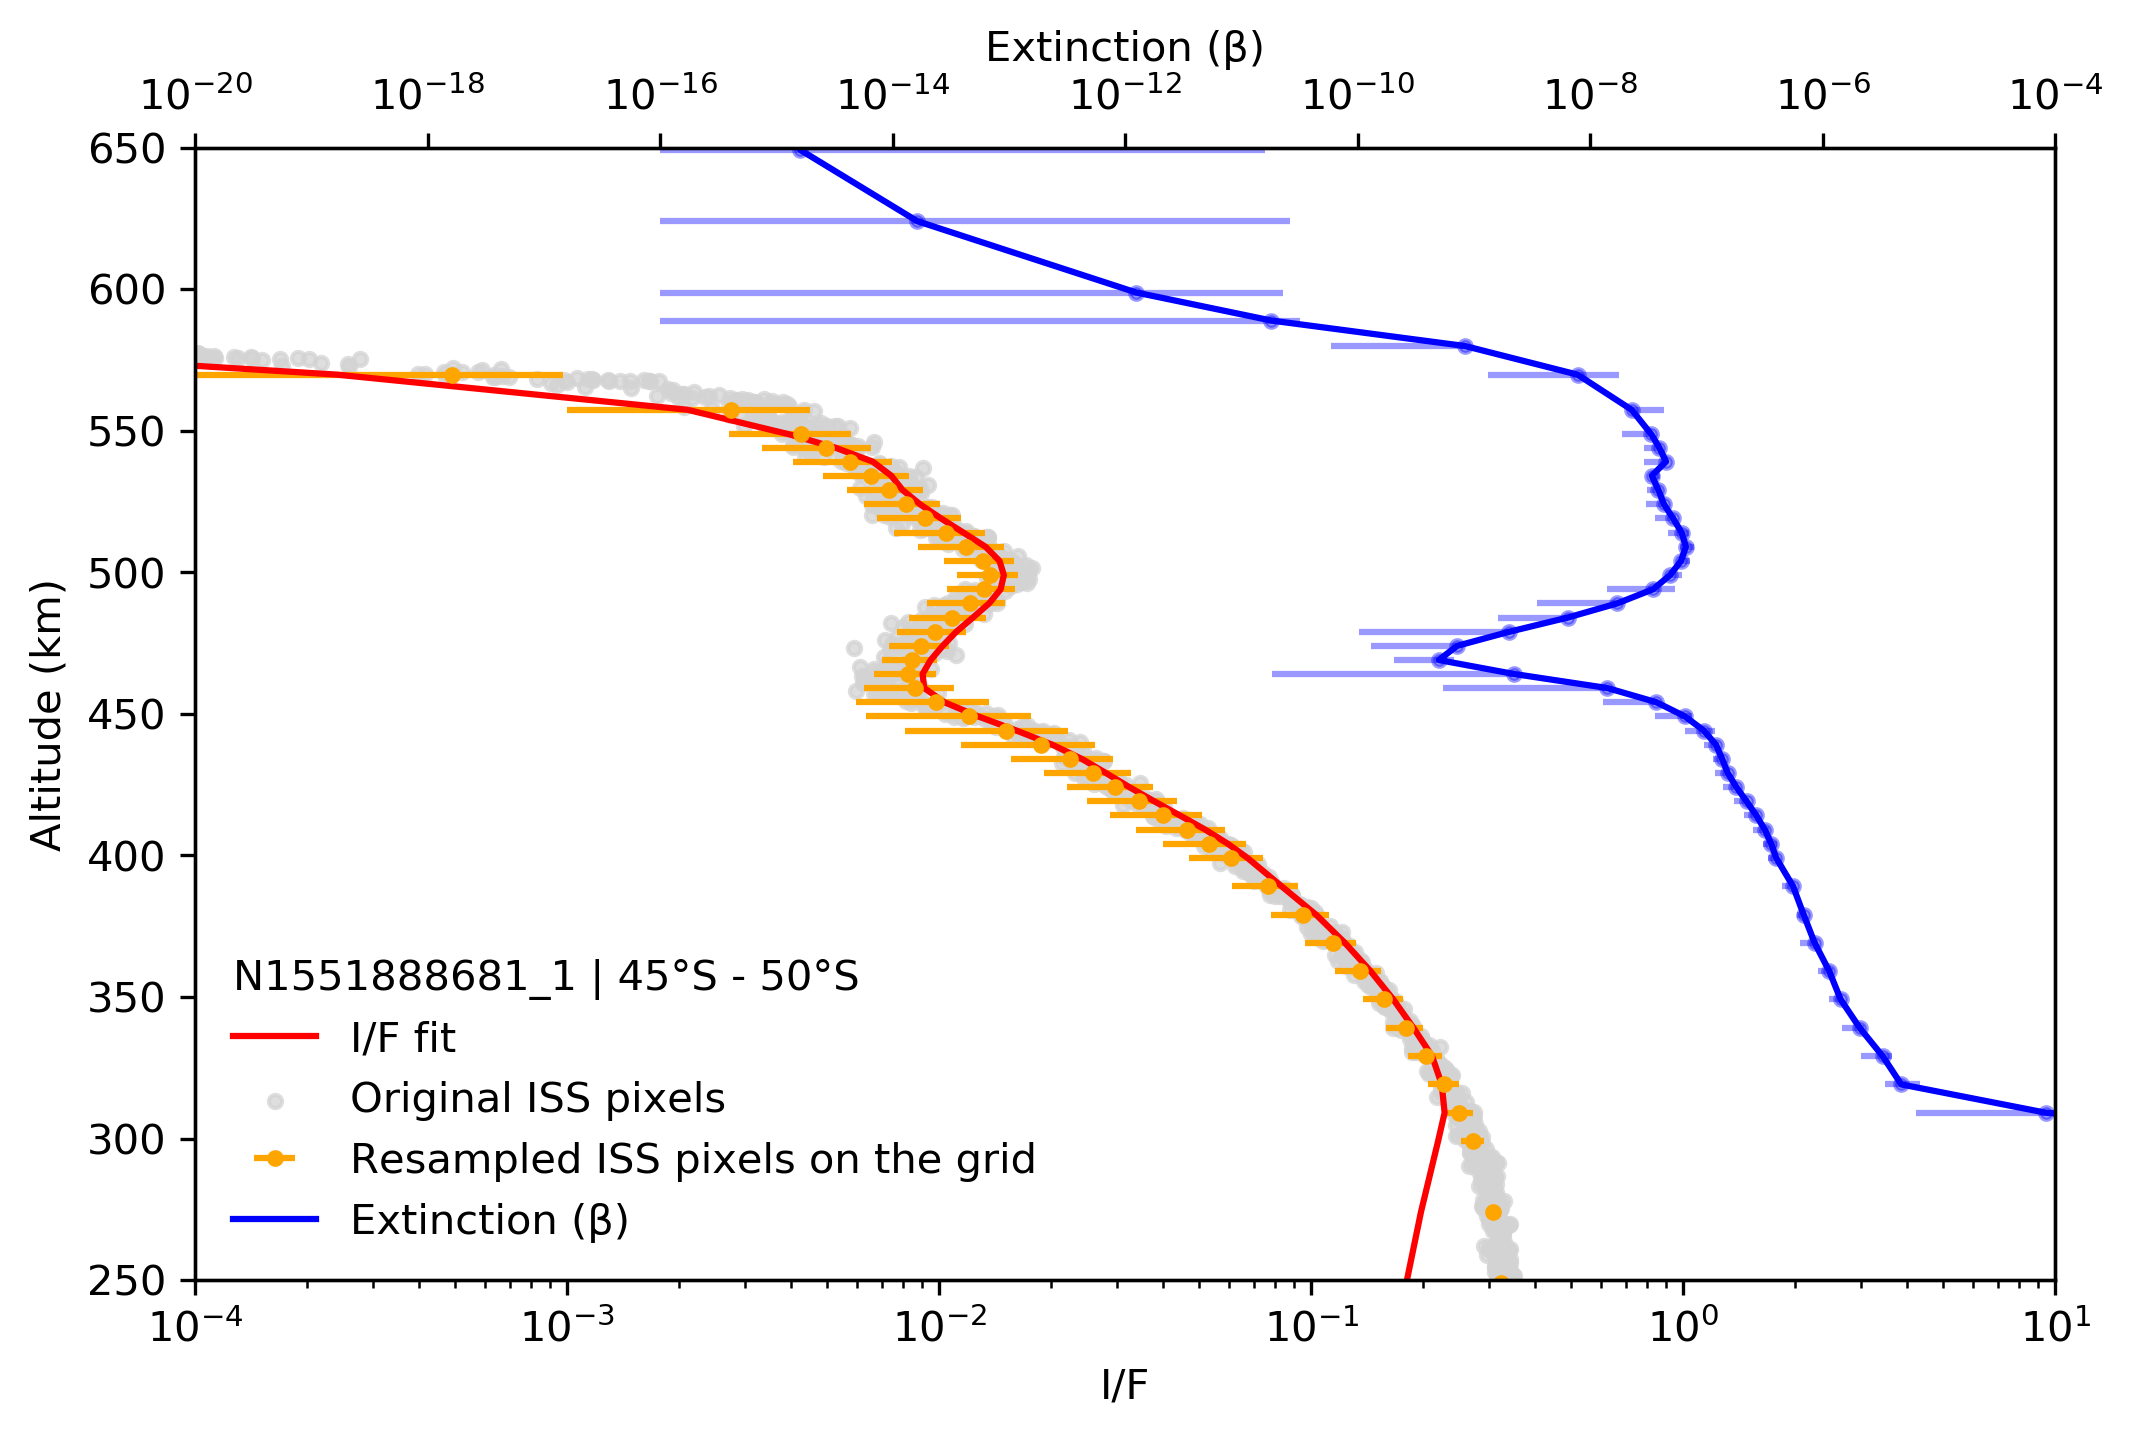
\includegraphics[height=6.5cm]{Fig/Model_uncertainties.png}
    \caption{Left: Log scale representation of the $I/F$  for the image
             \textbf{N1551888681\_1} taken in March, 2007. The data are sampled at the limb by
             bins of \ang{5}. The red area correspond to the bin at the photometric
             equator ([\ang{45}S, \ang{50}S] and [\ang{76}W, \ang{79}W]). The pixel scale
             (7.9 km/pixel) is represented in the zoomed area by the yellow rectangle.
             An altitude grid is also represented where we can see the peak of intensity of the DHL
             located at 500 km. Right: the red curve represents the inverted $I/F$ profile fitted
             on the resampled data (orange error bars). The uncertainties on the retrieved
             extinction profile $\beta$ (in blue) is calculated to match the $1 \sigma$ distribution
             of the $I/F$ pixels. The model fits the observations down to 300 km.
             The uncertainties increase rapidly when observed ($I/F$) is close
             to the noise level ($3\cdot10^{-3}$).}
    \label{fig:model_uncertainties}
\end{figure}

\section{Seasonal cycle of the haze extinction}

In order to provide a detailed explanation of the complex latitudinal variability of the detached haze layer, we present
some of the key images that we have analyzed. Based on the previous work focus on the evolution of the detached haze in the
equatorial region \citep{West2018}, we define four different phases characteristic of the evolution of the detached haze layer.
Between 2004 and 2008, the DHL was stable in altitude and extinction.
Between 2008 and 2012, it settled, merged and finally disappeared in the main haze.
During the period 2012-2016, the DHL was not observed and only sporadic transitory layers showed up.
After 2016 and up to the end of Cassini mission, the DHL reappeared following a complex pattern.
The complete survey is performed along a period of time which represents about half a Titan year.
This is valuable because it encompasses the equinoctial transition period of 2009.
For each phase, we display the altitude and latitude distribution of the instantaneous haze extinction retrieved from intensities at the illuminated limb of Titan.
The same color scale is applied to all the panels in order to keep a consistent view on the whole dataset.
Locations where no data are available are left as blank areas on the panels.

\subsection{Period 1: Stable detached haze Layer during the Northern Winter (2004-2008) - $L_s=\ang{300}-\ang{340}$}

At its arrival in the Saturnian system in 2004, Cassini observed a single detached haze layer at 500 km altitude 
(Fig.~\ref{fig:dhl_2004_2008}a) similar to the one observed at 350 km by Voyager 24 years before
\citep{Smith1981}. At that moment, Titan was two years after the winter solstice in the northern hemisphere, at $L_s=\ang{300}$.
With Cassini, we see that, in the southern hemisphere, the haze layer was completely detached from the main haze layer.
The haze extinction was at least one order of magnitude smaller inside the depleted zone (470 km) than in the main and
the detached haze layers (below 450 and at 500 km respectively).
Between the equator and up to about \ang{60}N it presented a local depletion in extinction
of a factor 10. There, the separation with the main haze is not as distinct as in the south, but is still sufficiently significant to
defined a detached haze layer.
The altitude of the depletion zone decreased by about 50 km between latitude \ang{30}N  and \ang{60}N.
The detached haze layer merged with the polar hood beyond \ang{60}N. This description of the detached haze layer at
the beginning of Cassini mission is very consistent with the results obtained from stellar occultation in 2003 \citep{Sicardy2006}.
Throughout the period 2004-2008 the detached haze layer was quite stable in shape and  altitude, with a maximum of extinction
at $500 \pm 20$ km. The top of the main haze layer was located around $450 \pm 20$ km below \ang{30}N and dropped
by 50 km between \ang{30} and \ang{60}N.

\begin{figure*}[!ht]
    \centering
    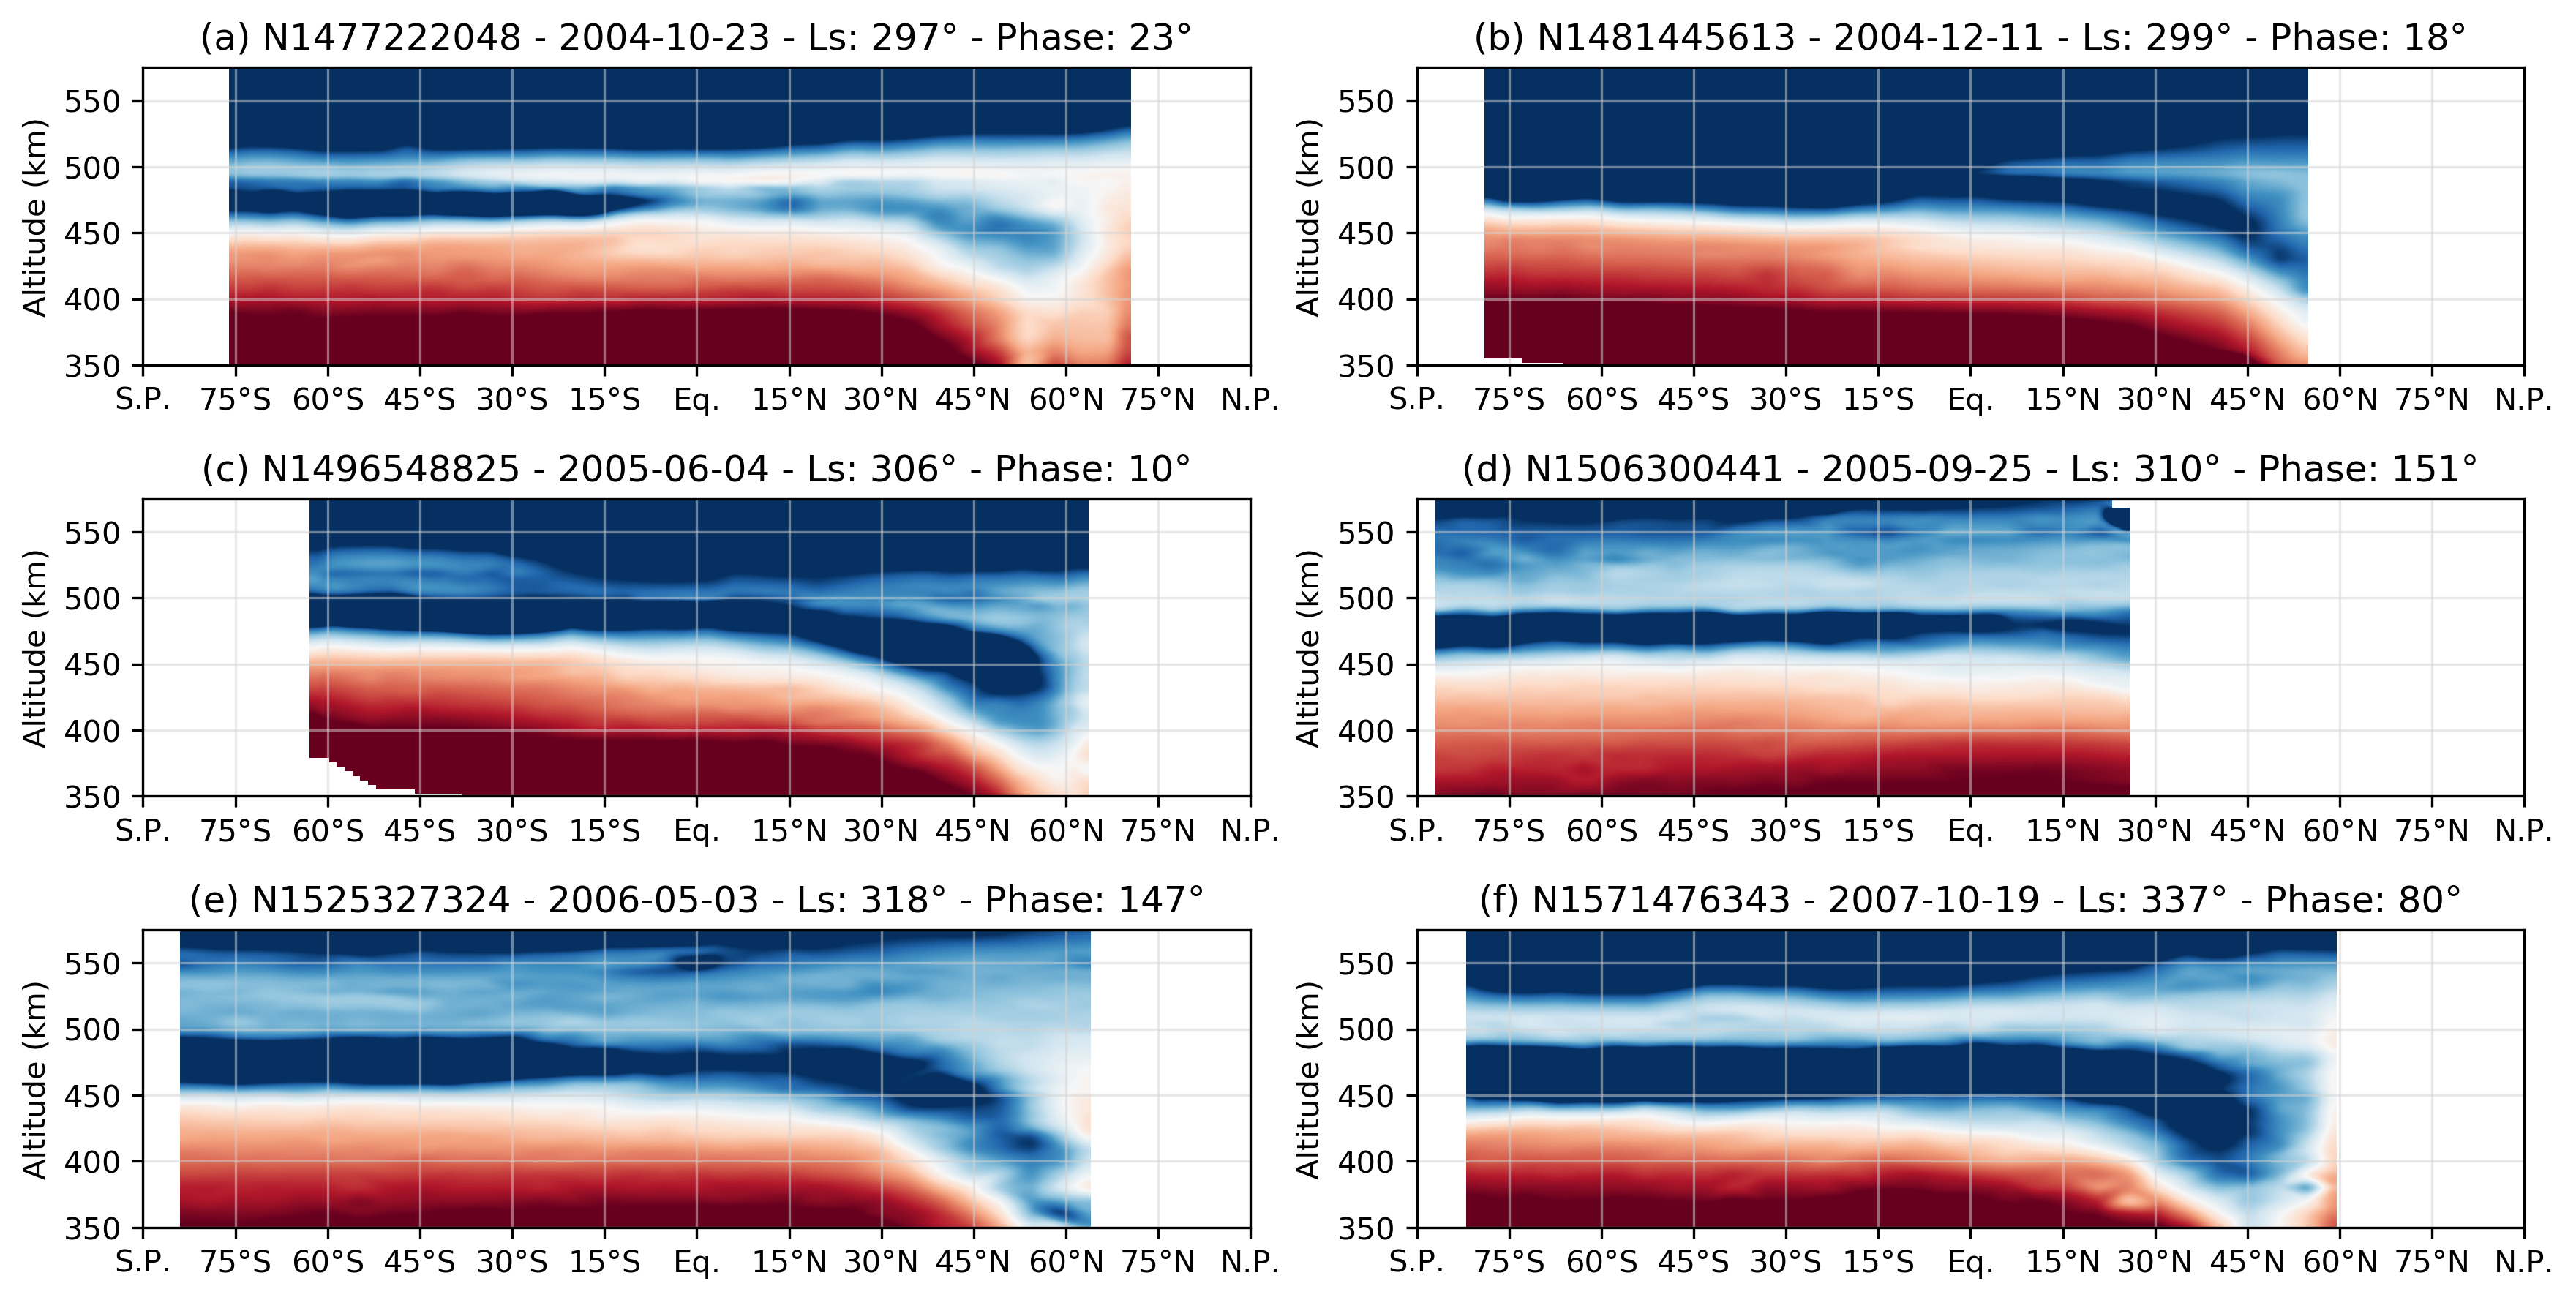
\includegraphics[width=\textwidth]{Fig/Lat_beta-2004_2008.png}
    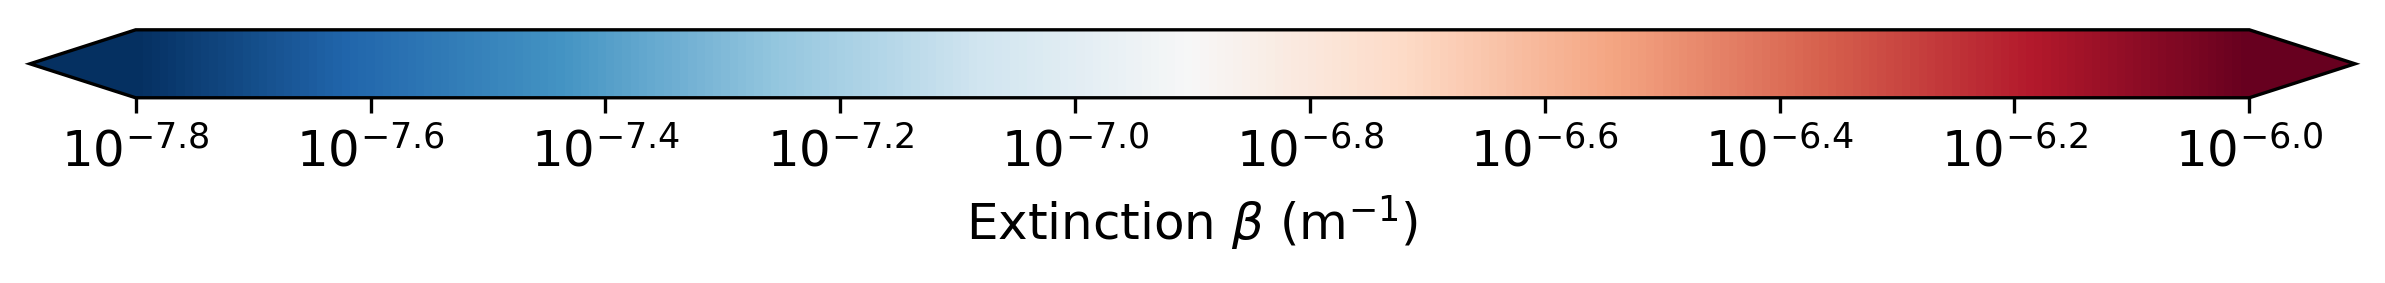
\includegraphics[width=.5\textwidth]{Fig/Extinction_colorbar.png}\vspace{-.3cm}
    \caption{Latitudinal haze extinction profile ($\beta$) retrieved for 6 images taken between 2004 and 2008
    ($L_s=\ang{300}-\ang{340}$) showing a stable DHL at $500 \pm 20$ km altitude.
    The color schema is fixed for all the figures to make direct comparison
    between the different panels. The seasonal solar longitude ($L_s$) and the observation phase angle are
    also provided in each panel.}
    \label{fig:dhl_2004_2008}
\end{figure*}

However, there are noticeable variations in haze extinction. During several months, the
detached haze remained stable, but in December 2004 (Fig.~\ref{fig:dhl_2004_2008}b),
the detached haze layer extinction was found to be a factor of 10 lower than previously at almost all latitudes south
of \ang{30}N, and about half a decade above \ang{30}N. The polar hood and the main haze do not show a similar decrease.
In the following periods, (Fig.~\ref{fig:dhl_2004_2008}c, d and e),
the detached haze was partially restored, but not with the same amount of extinction as before. Only observations in
2007 (Fig.~\ref{fig:dhl_2004_2008}f) show extinctions in the detached haze layer comparable to those seen before
the decrease. We note that the decrease of extinction below 370 km in the polar hood above \ang{50}N
(Fig.~\ref{fig:dhl_2004_2008}e) is at the limit of sensitivity of the UV filter. The stability of the large-scale
structure of the detached haze layer is related to the steady state of the large-scale circulation during all the winter.
The observation of October 2007 (Fig.~\ref{fig:dhl_2004_2008}f) is the last view that we have of this stable state
before the seasonal turnover.

During this period, the detached haze also has a strong layering with, at some latitudes, distinct decks which are not
continuous and rather appear as foliation. This feature is more pronounced in some observations, for instance from
June 2005 to May 2006, but does not shows up in October 2007, except marginally beyond \ang{30}N. The foliated detached
haze layer has a larger geometrical thickness than before December 2004.

% NOTE: [PR] We should really check that the apparent difference in geometric thickness of the DHL is not due to something else, as for instance, the phase angle. It could be due to a real effect of some aerosols above the DHL which scatter in a different way than aerosols in DHL itself. Or it could be due to a deconvolution effect that could differ depending on the appearance of Titan as a full disk or a crescent...

As we will see in the \textbf{section 4}, the detached haze layer exhibits some longitudinal or diurnal variability
that limits our ability to interpret details of features observed in single images. The small-scale features
could depend on the local short-term dynamics such as initia-gravity waves.

\subsection{Period 2: Drop and disappearance of the main haze layer around the Vernal Equinox (2008-2012) - $L_s=\ang{340}-\ang{30}$}

A precursor sign of the drop of the detached haze can be seen in March 2008 (Fig.~\ref{fig:dhl_2008_2012}a).
The main haze starts an initial contraction, perceptible around \ang{35}S. There, the depleted zone is almost
75 km thick at its maximum. In January 2009, the main haze continued to fall down from 425 km down to 375 km
while the detached haze layer remained around 500 km (Fig.~\ref{fig:dhl_2008_2012}b). After the drop
of the main haze in early 2009, the detached haze starts its own descent in June 2009, just before the equinox
(Fig.~\ref{fig:dhl_2008_2012}c). This delay in collapse increased the apparent thickness of the depletion
zone between the two haze layers.

\begin{figure*}[!ht]
    \centering
    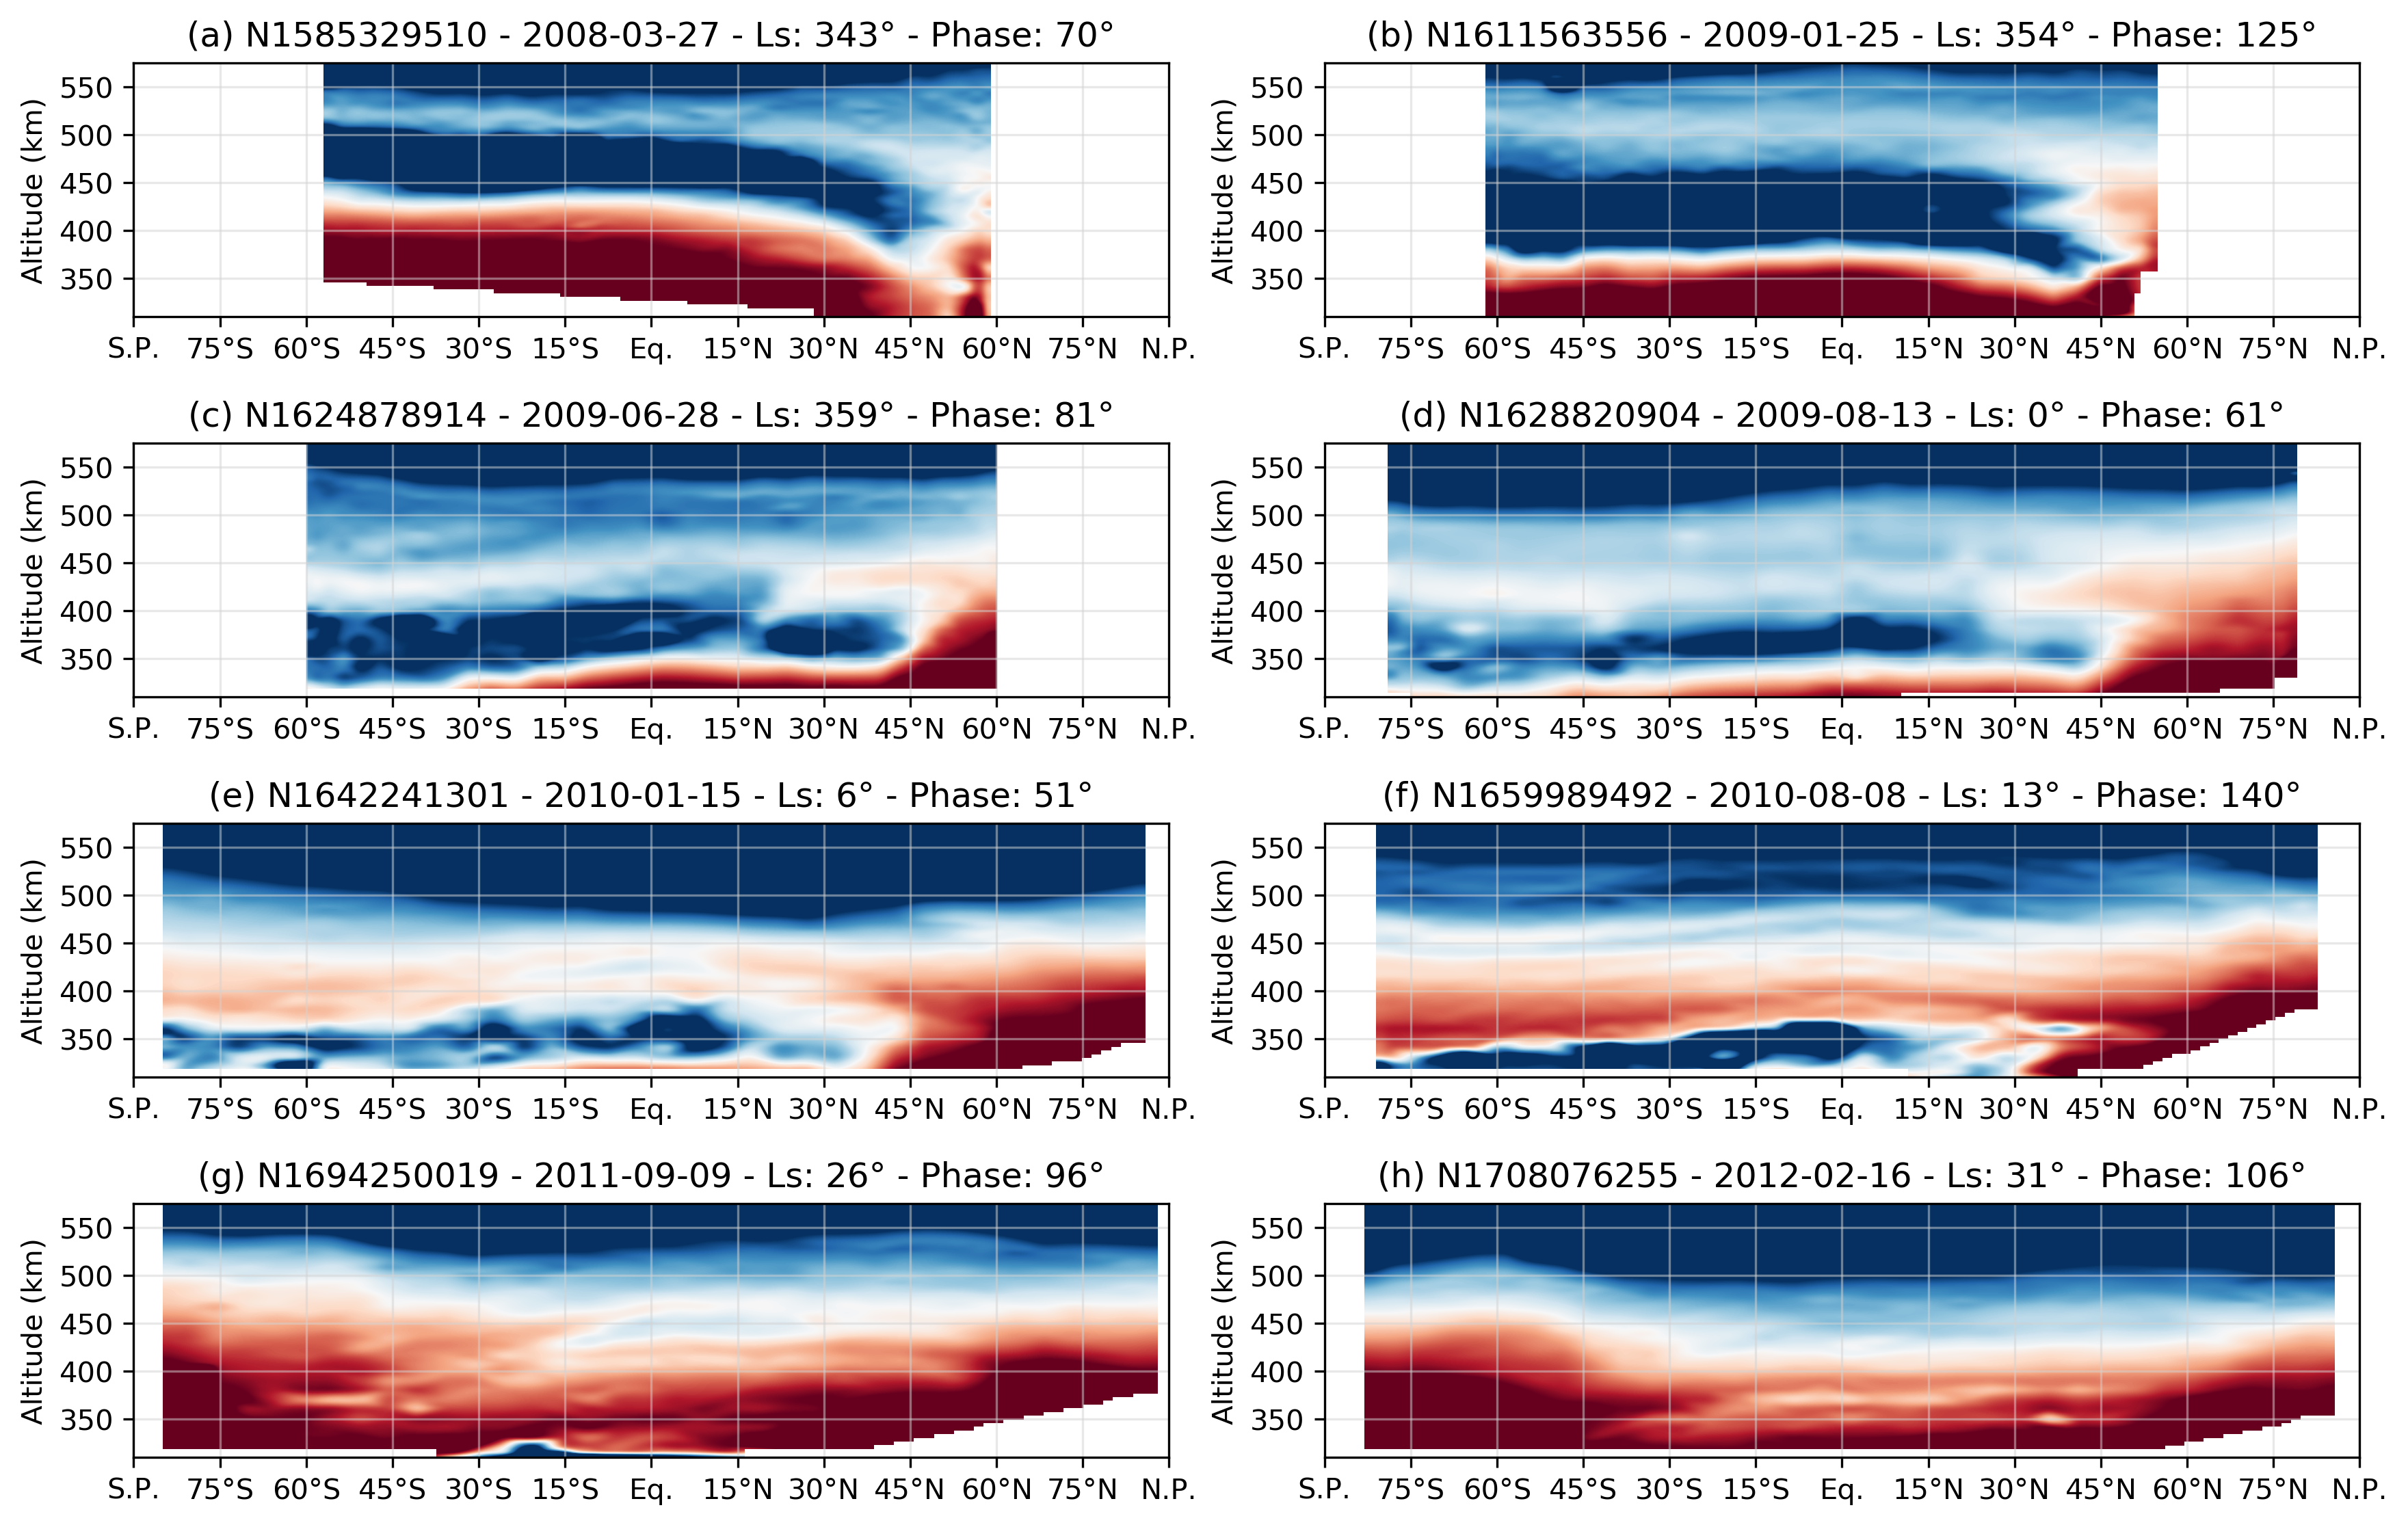
\includegraphics[width=\textwidth]{Fig/Lat_beta-2008_2012.png}
    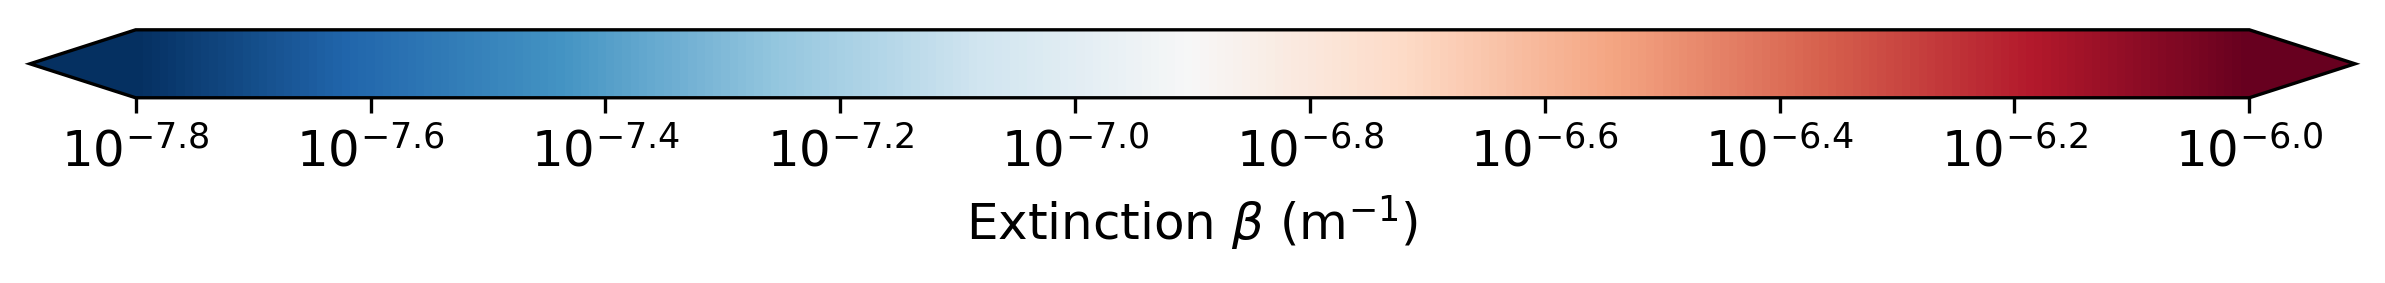
\includegraphics[width=.5\textwidth]{Fig/Extinction_colorbar.png}\vspace{-.3cm}
    \caption{Same as the figure~\ref{fig:dhl_2008_2012} for 8 images taken between 2008 and 2012
    ($L_s=\ang{340}-\ang{30}$) showing the collapse of drop and disappearance of the DHL.
    The color schema extent is kept similar to the figure~\ref{fig:dhl_2008_2012} to provide
    direct comparisons but the altitude range is extended down to 300 km around the UV3 saturation
    level (where the atmosphere is opaque).}
    \label{fig:dhl_2008_2012}
\end{figure*}

As for the main haze, the detached haze collapses first in the South hemisphere, from 500 km to 425 km, and
then at equator and in the northern hemisphere (Fig.~\ref{fig:dhl_2008_2012}c).
This is associated to the circulation turnover affecting first the summer hemisphere ascending branch.
With time, the detached haze gradually settled in altitude and finally merged with
the main haze. The complete collapse of the detached haze is displayed in Fig.~\ref{fig:dhl_2008_2012}c to
Fig.~\ref{fig:dhl_2008_2012}h. We note that the extinction of the detached haze is smaller at equator than at
other latitudes, and this will be the case during all the drop.

During the fall, a second thin detached haze layer, at planetary scale, can be remarked above the collapsing detached
haze layer. In January 2010 (Fig.~\ref{fig:dhl_2008_2012}e), the detached is now located between 375 and 400 km.
We can still see a double deck of haze, and this time the detached haze appears higher at the equator compare to the two
hemispheres, producing an arch. The haze extinction has globally increased by a factor of two due to sedimentation
in denser layers.

In August 2010 (Fig.~\ref{fig:dhl_2008_2012}f), one year after equinox, the detached haze layer continued
its drop down to 350 km around \ang{40}N and 400 km at the equator. It has gained in complexity with
multiple secondary layers up to 520 km. The detached haze form a remarkable arch with a difference of about 50 km
in altitude between the equator and the poles as previously noticed by~\cite{West2011}.
This observation and the next one correspond to the same time of the
year than the time of Voyagers flybys ($L_s=\ang{8}$ and \ang{18}). They can be compared quite directly. We now know
that this season was a time of rapid change, and that the Voyager probes observed transient situations. Voyager also
observed the detached haze higher near equator than elsewhere \citep{Rages1983, Rannou2000}. This corresponds to
the detached haze layer following an isobar level.

Due to orbital constrain and mission planning, the next observation was made in September 2011
(Fig.~\ref{fig:dhl_2008_2012}g). The detached haze layer is now well below the level of the polarhoods.
Again secondary detached layers show up as high as 470 and 520 km.
The south polarhood was not present in January 2010 (Fig.~\ref{fig:dhl_2008_2012}e), it could not be seen
neither northward to \ang{70}S in August 2010 (Fig.~\ref{fig:dhl_2008_2012}f). We conclude that it was surely
built in less than 20 months, and may be less than seven months. The circulation started to reverse around the equinox
and the southward circulation send haze in the south pole and produced this polarhood. The change in haze distribution
is a very good indication of the timing of the equinoctial circulation turnover, has it is discussed later. We note
that the strong haze depletion at 300 km and between \ang{30}S and \ang{20}N is real but may be exaggerated at \ang{20}N
due to the limit of the retrieval procedure. At this altitude level, Titan's atmosphere is opaque to UV radiations
(see Fig.~\ref{fig:model_uncertainties}) and does not allow use to follow the main depletion below this altitude.

The last image that we have with a detached is February 2012 (Fig.~\ref{fig:dhl_2008_2012}h). At that
time, the initial detached haze has completely disappeared and the secondary detached hazes is still descending
and reach 400 km. The secondary detached hazes is not well delineated by a layer strongly depleted in aerosols.
The south polarhood increases its latitudinal extent northward to \ang{50}S and becomes larger than the northern
polarhood which tends to decrease.

\subsection{Period 3: Absence of DHL with sporadic transitory layers after the Northern Spring Equinox (2012-2015) - $L_s=\ang{30}-\ang{75}$}

During this period, the main haze layer has large scale structures which slowly evolve under the influence of the
large scale circulation. The south and north polarhoods are still visible and they evolve
with time. Superimposed to this background haze, transient structures show up and disappear from one observation
to the other. At some moments, large scale detached hazes appear. They differ from the detached haze seen at the
beginning of the mission because they are not stable in time and in altitude. They do not appear from one
observation to the other. The haze during this period is displayed in Fig.~\ref{fig:dhl_2012_2015}.

\begin{figure*}[!ht]
    \centering
    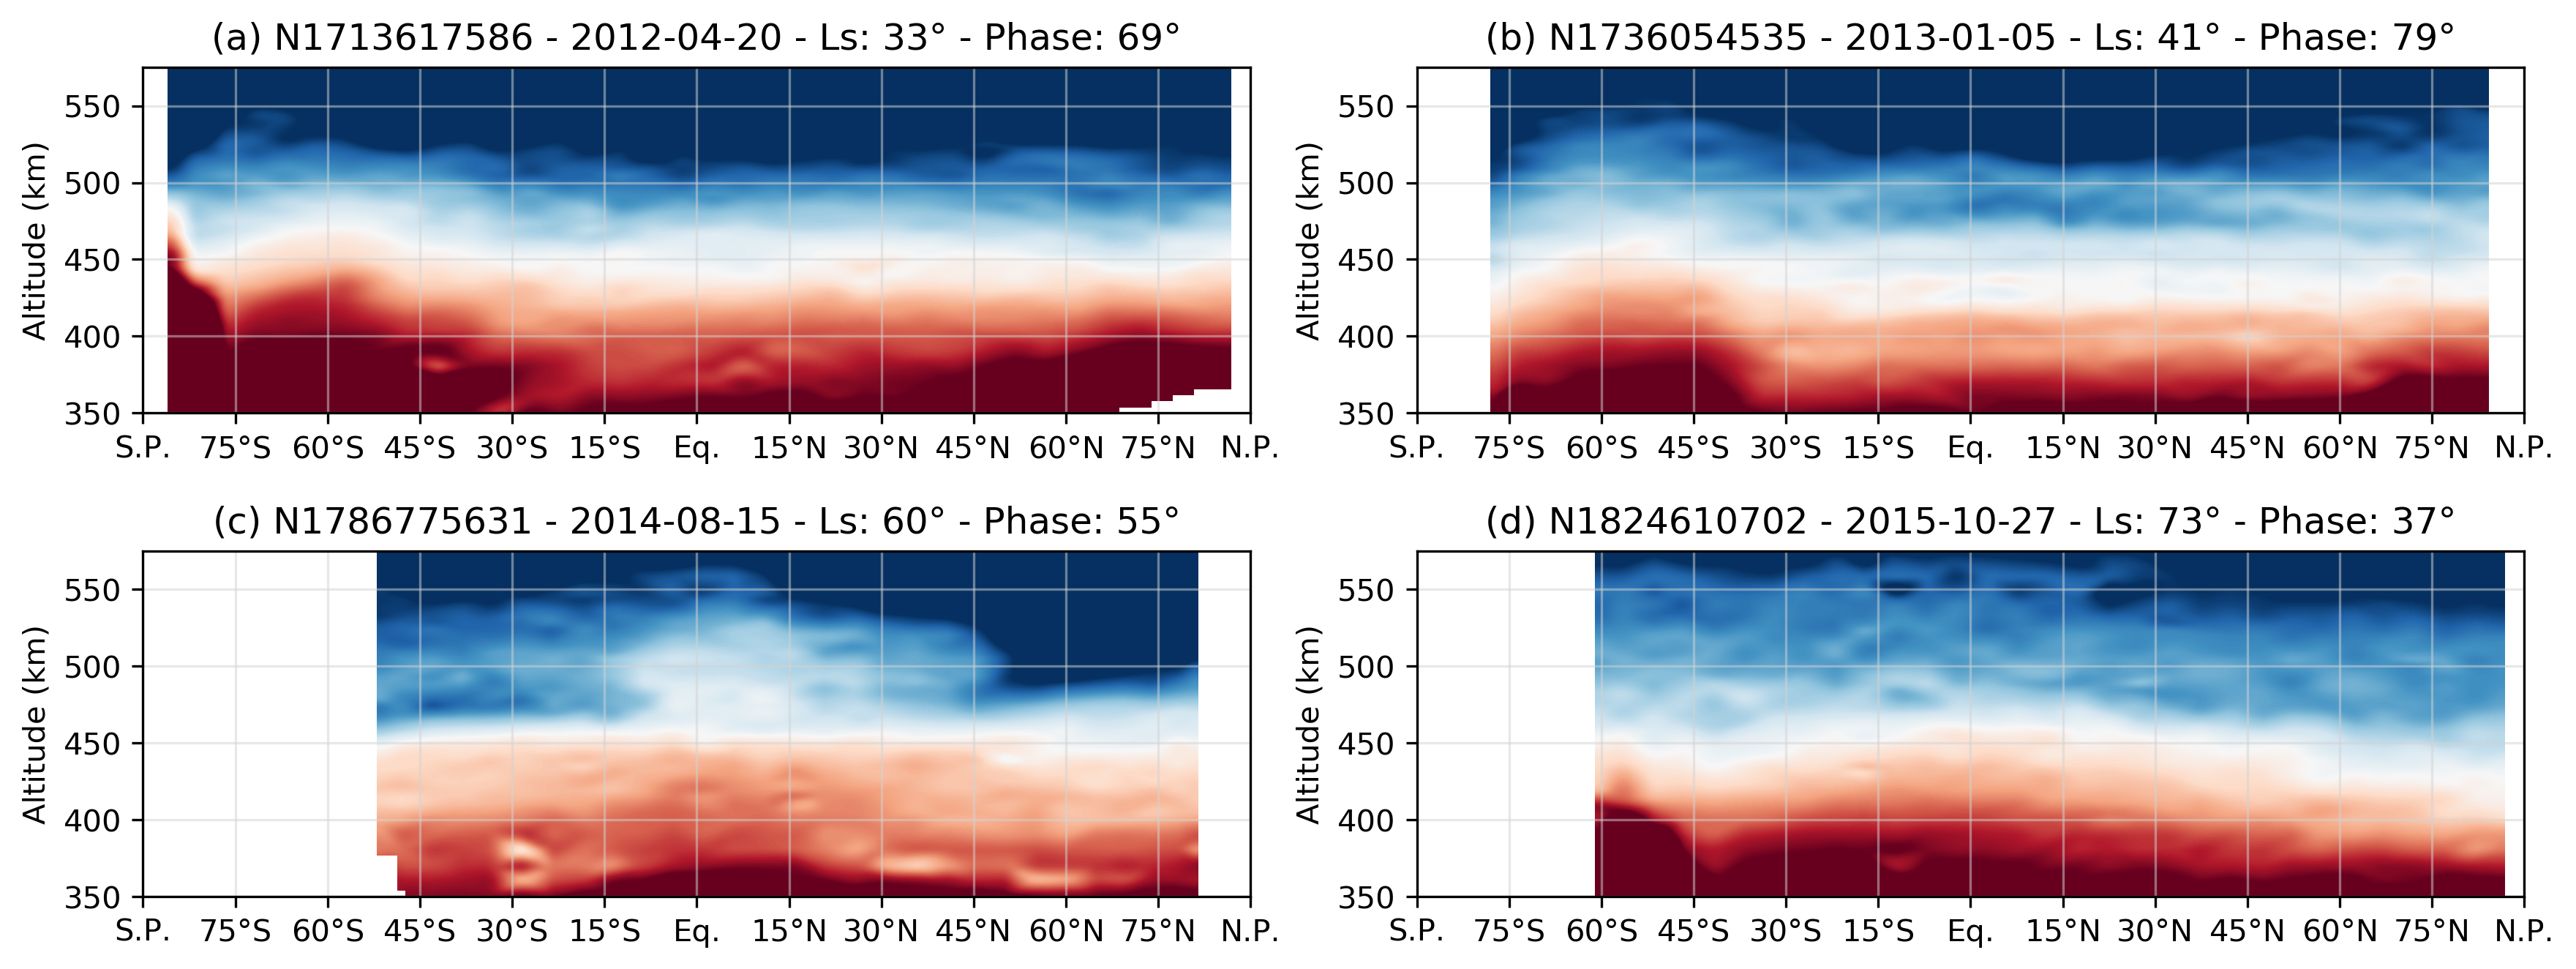
\includegraphics[width=\textwidth]{Fig/Lat_beta-2012_2015.png}
    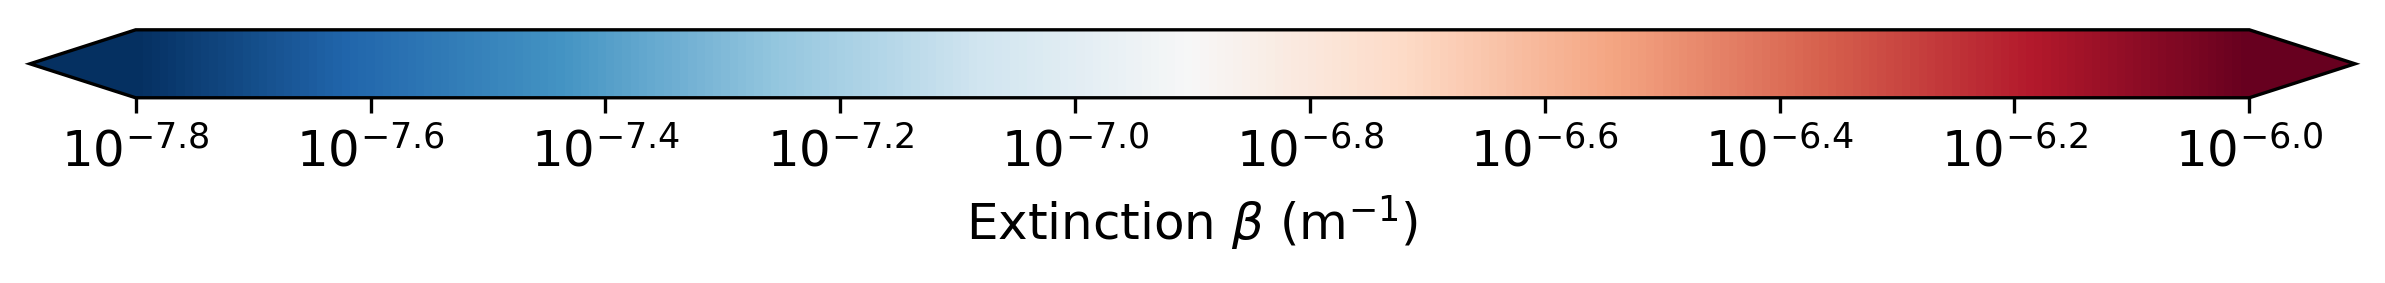
\includegraphics[width=.5\textwidth]{Fig/Extinction_colorbar.png}\vspace{-.3cm}
    \caption{Same as the figures~\ref{fig:dhl_2004_2008} and~\ref{fig:dhl_2008_2012}
    for 4 images taken between 2012 and 2015 ($L_s=\ang{30}-\ang{75}$) showing sporadic
    transitory layers and the absence of consistent DHL.
    The color extent is the same and the altitude ranges down to 350 km.}
    \label{fig:dhl_2012_2015}
\end{figure*}

In April 2012 (Fig.~\ref{fig:dhl_2012_2015}a), the detached haze has completely disappeared, except a residual
structure at \ang{5}-\ang{20}S, around 370 km.
This relict of the last detached haze layer is almost not perceptible in the corresponding I/F profile. At other
latitudes, we only can see a unique main haze with a marked south polarhood and a small increase of extinction above
\ang{65}N that could be the north polarhood. Sometimes, detached layers emerge from the background with large latitudinal
extent (e.g. detached haze at 500 km Fig.~\ref{fig:dhl_2012_2015}b). However, they only remain for a short time
and are not seen in the following observations.

In August 2014 (Fig.~\ref{fig:dhl_2012_2015}c) we observed a plume of aerosol between \ang{10}S and \ang{25}N,
at 500 km. A detached haze layer seems to have spread from this plume toward the north and the south. This
detached haze is around 500 km, descending to 470 km at \ang{60}S (and probably even southern). At the
north, the detached haze does not extend northern than \ang{50}N and remains at 500 km. This indicate an
atmosphere circulation rather flowing from equator toward the south pole. The origin of these aerosols is undefined.

The observation of October 2015 (Fig.~\ref{fig:dhl_2012_2015}d) is very representative of the haze layer in
the period between 2012 and the end of 2015. At this date, the main haze has a uniform scale height of 45 km and
with a homogenous extinction at the planetary scale.

\subsection{Period 4: Reappearance of a new detached haze layer around the Summer Solstice (2015-2017) - $L_s=\ang{75}-\ang{95}$}

The first occurrence of the detached haze in this period is the 3$^{rd}$ December 2015
(Fig.~\ref{fig:dhl_2015_2017}a). Strictly speaking, it
does not differ from the previous sporadic detached haze layers observed in the period 2012-2015. But, after
this observation, the detached haze was present in each observations. The detached haze became stable in time,
similarly to the detached haze before the equinox. Therefore, we consider this date as the beginning of the
reappearance of the detached haze ($L_s=\ang{74}$). The evolution of the haze during this period is displayed in
Fig.~\ref{fig:dhl_2015_2017}. The observations validate the long awaited reappearance of the detached haze layer,
just before the end of the Cassini mission in September 2017.

\begin{figure*}[!ht]
    \centering
    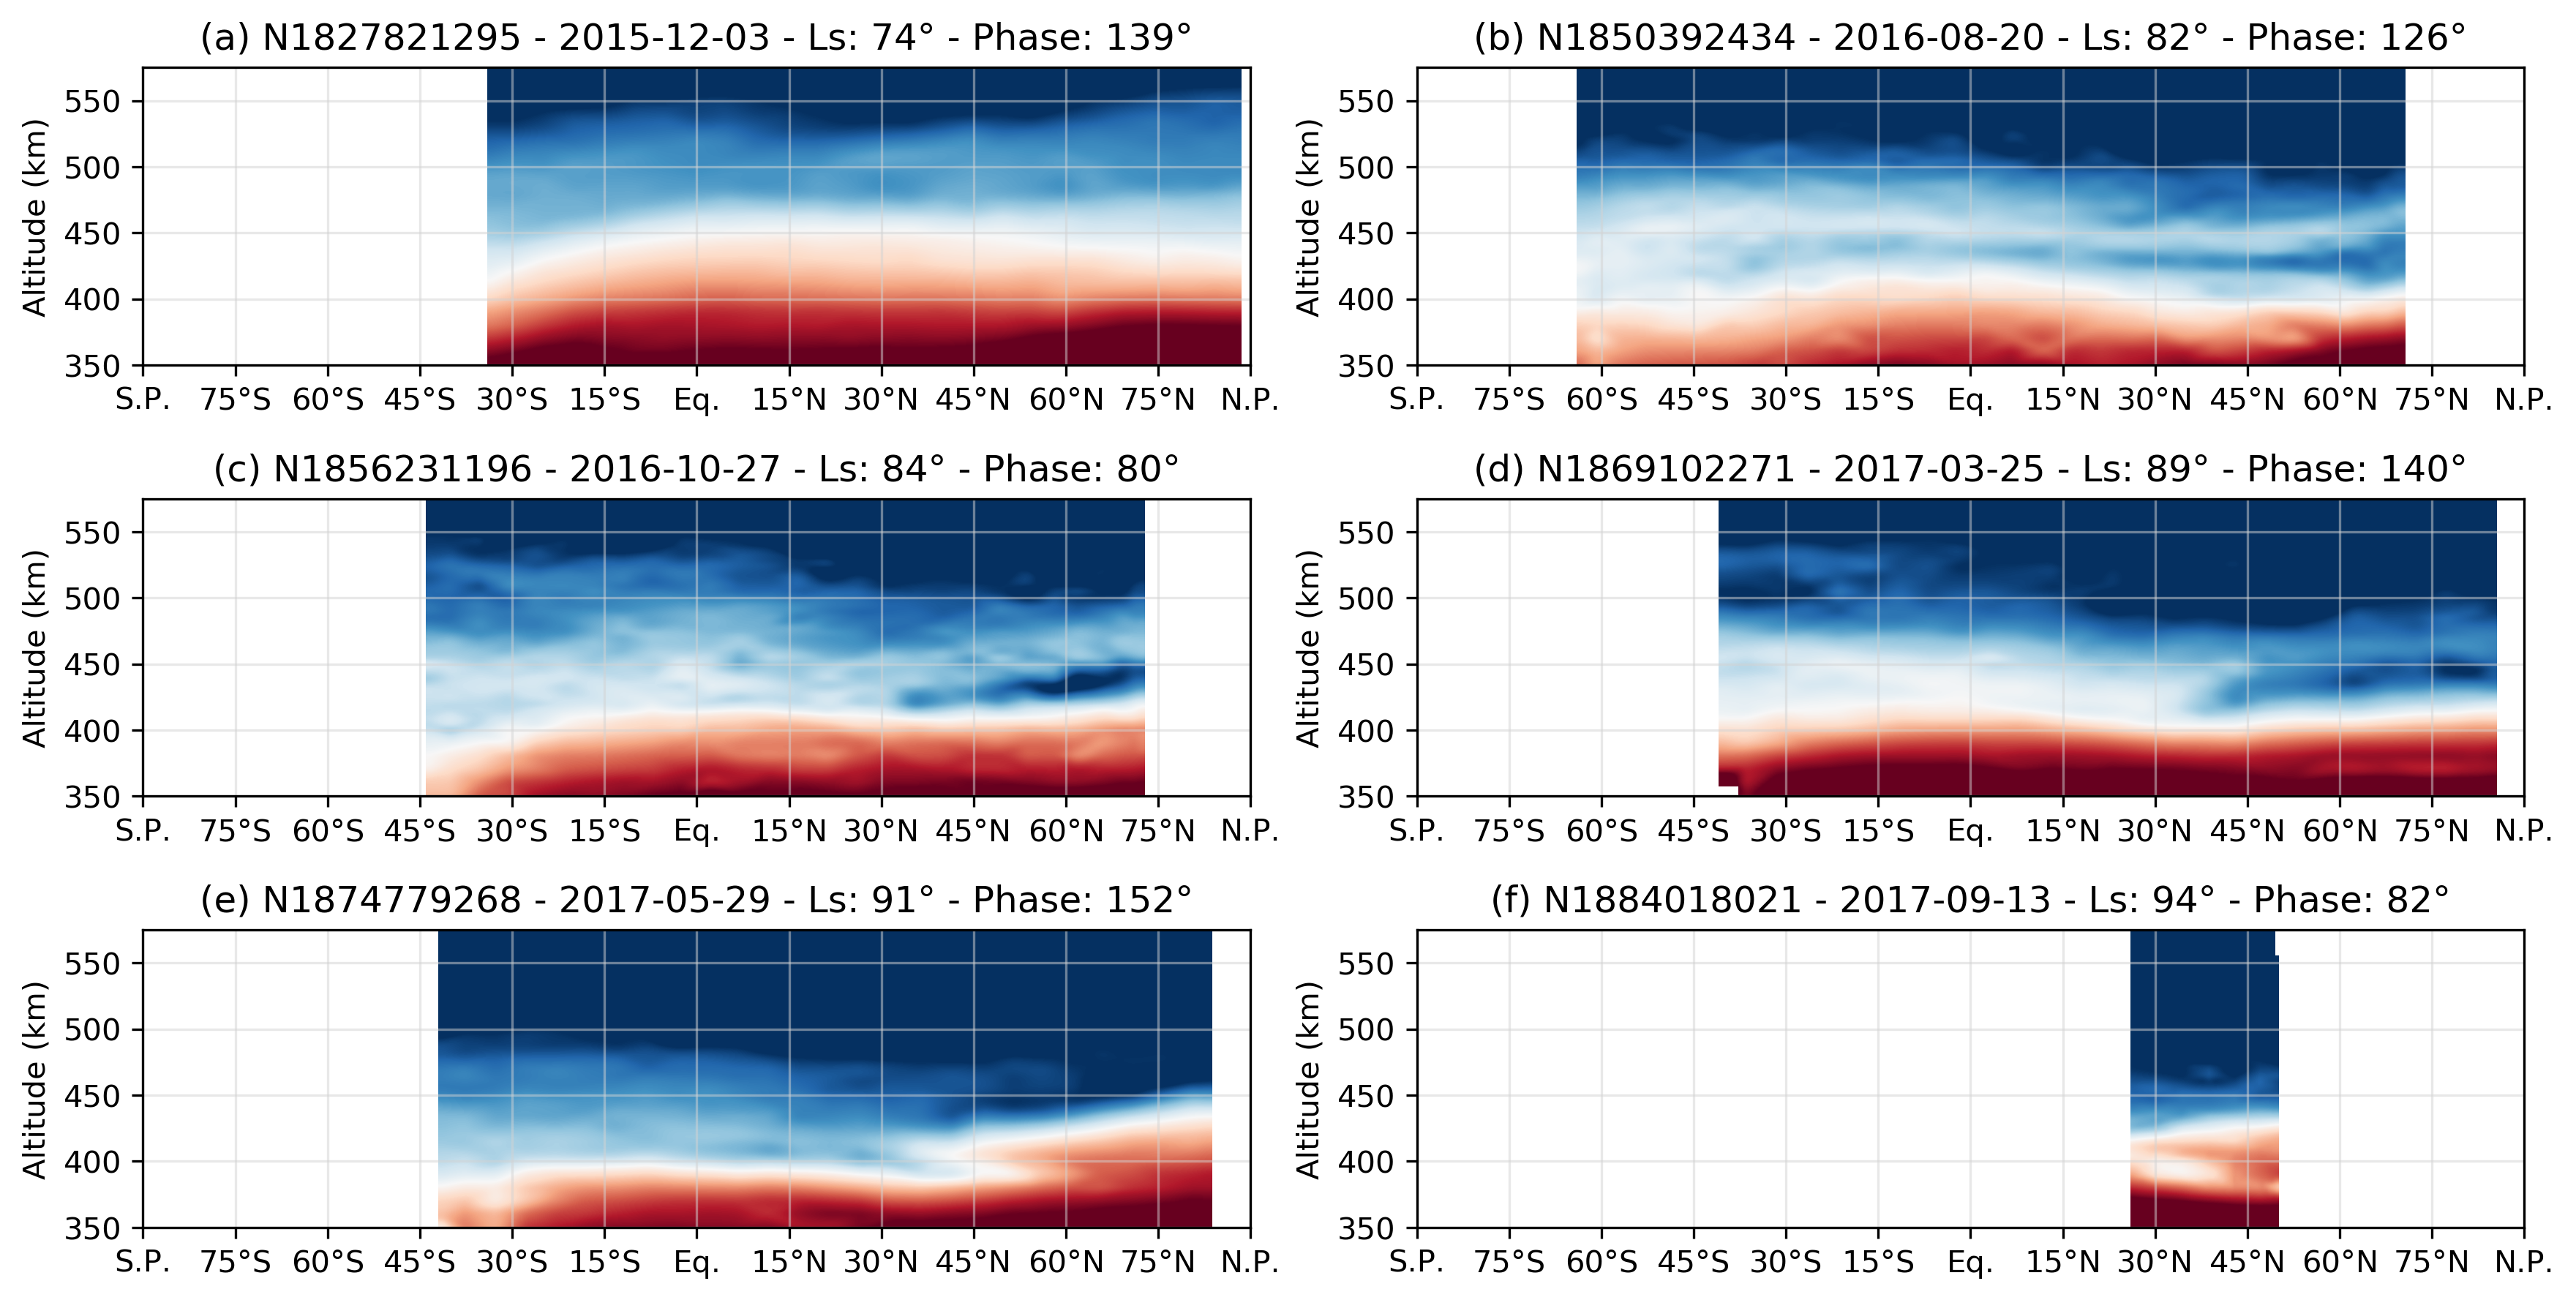
\includegraphics[width=\textwidth]{Fig/Lat_beta-2015_2017.png}
    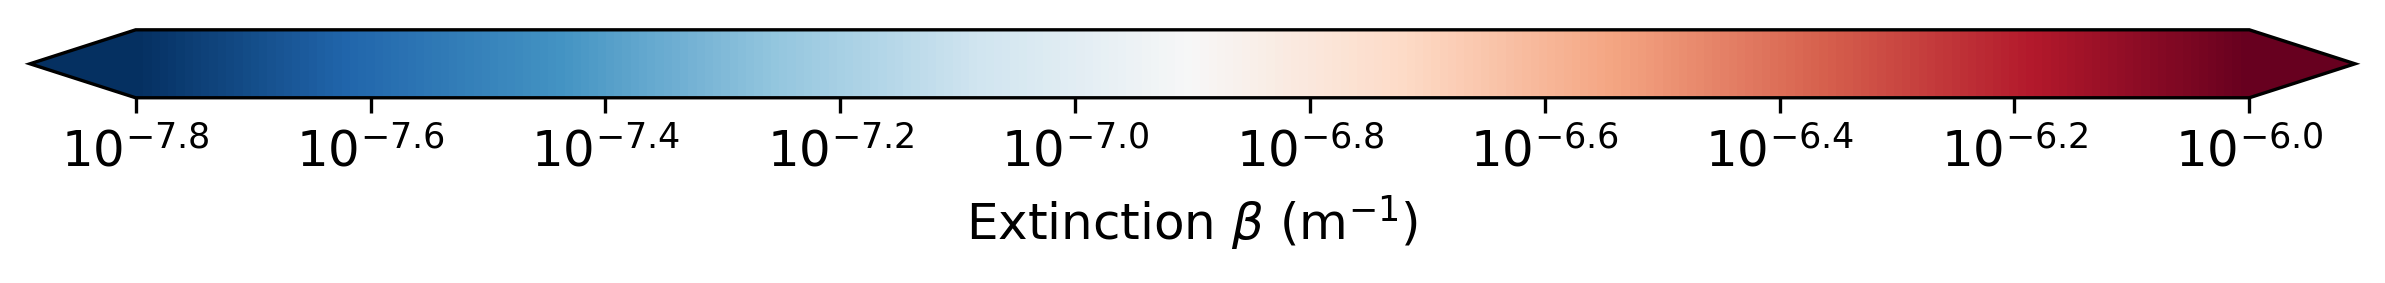
\includegraphics[width=.5\textwidth]{Fig/Extinction_colorbar.png}\vspace{-.3cm}
    \caption{Same as the figures~\ref{fig:dhl_2004_2008}, \ref{fig:dhl_2008_2012}
    and~\ref{fig:dhl_2012_2015} for 6 images taken between 2015 and 2017
    ($L_s=\ang{75}-\ang{95}$) during the reappearance of the DHL.
    The image \textbf{N1884018021\_1} is one of the very last observation of Titan before
    the end of the Cassini mission in September 2017.}
    \label{fig:dhl_2015_2017}
\end{figure*}

At the beginning, the detached haze layer is not very well defined but it can be perceived at all latitudes
around 490 - 520 km (Fig.~\ref{fig:dhl_2015_2017}a). We notice at the same moment a contraction
the main haze, with the top of the haze dropped by 50 km in January 2016 compared to October 2015
(Fig.~\ref{fig:dhl_2012_2015}d). The main elements of the reappearance (altitude and date) confirms the
predictions made by the general circulation models \citep{Lebonnois2012,Larson2015} and the prediction
reported in \cite{West2011}. The detailed comparison between the observations and GCM is discussed further.

With time, the detached haze layer is better marked and the zone of depletion is more pronounced, especially in the
northern hemisphere (Fig.~\ref{fig:dhl_2015_2017}b). The situation seems to be analogue to an early stage of
the structure observed in 2004 (with the opposite latitude). However, although the detached haze persists in time,
it also settles and almost merges with the main haze in October 2016 (Fig.~\ref{fig:dhl_2015_2017}c).
In the  following observations (Fig.~\ref{fig:dhl_2015_2017}d and Fig.~\ref{fig:dhl_2015_2017}e), we are
witnessing the complex evolution of the first appeared detached haze that merge with the main layer at latitude southward
to $\simeq \ang{35}$N while it remains stable around 450 km northward to \ang{35}N and seems to vanish rather than settle.
This structure was still observed in the very last image of Titan taken by Cassini just before its last plunge into Saturn
atmosphere (Fig.~\ref{fig:dhl_2015_2017}f) in September 2017.

A secondary detached haze layer appears in the southern hemisphere at high altitude around 520 km
(Fig.~\ref{fig:dhl_2015_2017}c). Its northern boundary is not well defined. This new structure will be persistent with
time, at planetary scale up to the end of Cassini mission but is gradually descending. The results reported by \cite{West2018}
concerns the detached haze at equator only. Although they already revealed a complex behavior of the detached haze layer, the
present observations show a dichotomy between the two hemispheres. The detail of the evolution, the split in a double layer
structure, the formation and disappearance of several structures was completely unexpected. According to GCMs, six years
after equinox, the post-equinoctial circulation was supposed to be already installed with a planetary scale circulation cell
from the south hemisphere to the north polar region. Apparently, this is not the case.

These observations from 2004 to 2017 does not completely cover half a Titan year. The first and last observations
were taken almost at the opposite season, $L_s=\ang{297}$ and \ang{94} respectively (\emph{i.e.} \ang{157} apart).
This prevents direct comparisons between the detached haze at the beginning and at the end of the mission,
although in both cases they are taken more than a season after the previous solstice.

\section{Local and short-term variability of the detached haze layer}

So far, we have considered the evolution of the detached haze layer in the frame of the seasonal change.
We then discussed the long term-evolution at the planetary scale as a function of latitude.
In this section we consider sets of observations to characterize short-term \change{and local} behavior of the detached haze.
\change{These characterizations could only be conducted on a limited number of observations and require very specific acquisition geometries. They allow us to observe localized, secondary order variations of the detached haze layer.}
First, we choose several images taken a few hours apart to
evaluate the hourly variability of the detached haze. Next, we consider
observations at low phase angle which show simultaneously the two limbs of Titan. And, finally,
we consider observations taken from a near-polar point of view which can show
longitudinal variations in a narrow range of latitudes.

\subsection{Short time or spatial  variability}

As presented before, we observe between December 2004 and June 2005 a large amplitude variability of the
detached haze layer extinction profile at all the latitudes below \ang{35}N (Fig.~\ref{fig:dhl_2004_2008}a
to \ref{fig:dhl_2004_2008}c). Fortunately, Cassini took in June 2005 a series of 9 images of
Titan with a time-step of 80 minutes apart (Table.~\ref{tab:time_variability}).

\begin{table}[!ht]
    \centering
    \caption{Sequence of the 9 images of Titan taken June 4$^{th}$, 2005.
    The longitude and local time are given for the profile at the equator
    on the illuminated side of Titan.}
    \vspace{.5cm}
    \begin{tabular} {c c c c c}
        \toprule
        Imag ID & Time (UTC) & Phase & Longitude (Eq) & Local Time (Eq)\\
        \midrule
        N1496548825\_1 & 03:32 & \ang{10.4} & \ang{10.7}W & 17:12 \\
        N1496552665\_1 & 04:36 & \ang{10.3} & \ang{10.4}W & 17:17 \\
        N1496557465\_1 & 05:56 & \ang{10.1} & \ang{10.6}W & 17:23 \\
        N1496562265\_1 & 07:16 &  \ang{9.9} & \ang{13.1}W & 17:17 \\
        N1496567065\_1 & 08:36 &  \ang{9.8} & \ang{13.4}W & 17:23 \\
        N1496571865\_1 & 09:56 &  \ang{9.8} & \ang{13.9}W & 17:23 \\
        N1496576665\_1 & 11:16 &  \ang{9.8} & \ang{14.3}W & 17:30 \\
        N1496581465\_1 & 12:36 &  \ang{9.9} & \ang{14.7}W & 17:30 \\
        N1496586265\_1 & 13:56 & \ang{10.1} & \ang{15.2}W & 17:36 \\
        \bottomrule
        \label{tab:time_variability}
    \end{tabular}
\end{table}

With multiple observations of Titan in a short period, we are able to validate our calibration and
observe short time and local variabilities. Here, we analyze the sequence at three different
locations on the limb (\ang{40}S, \ang{0}, \ang{40}N). The 9 observations are made with phase
angles around \ang{10}, within an interval of \ang{0.6}. The limb longitude of the observations
varies  between \ang{10}W and \ang{15}W whereas the solar local time on Titan varies between
17:12 and 17:36.

\begin{figure}[!ht]
    \centering
    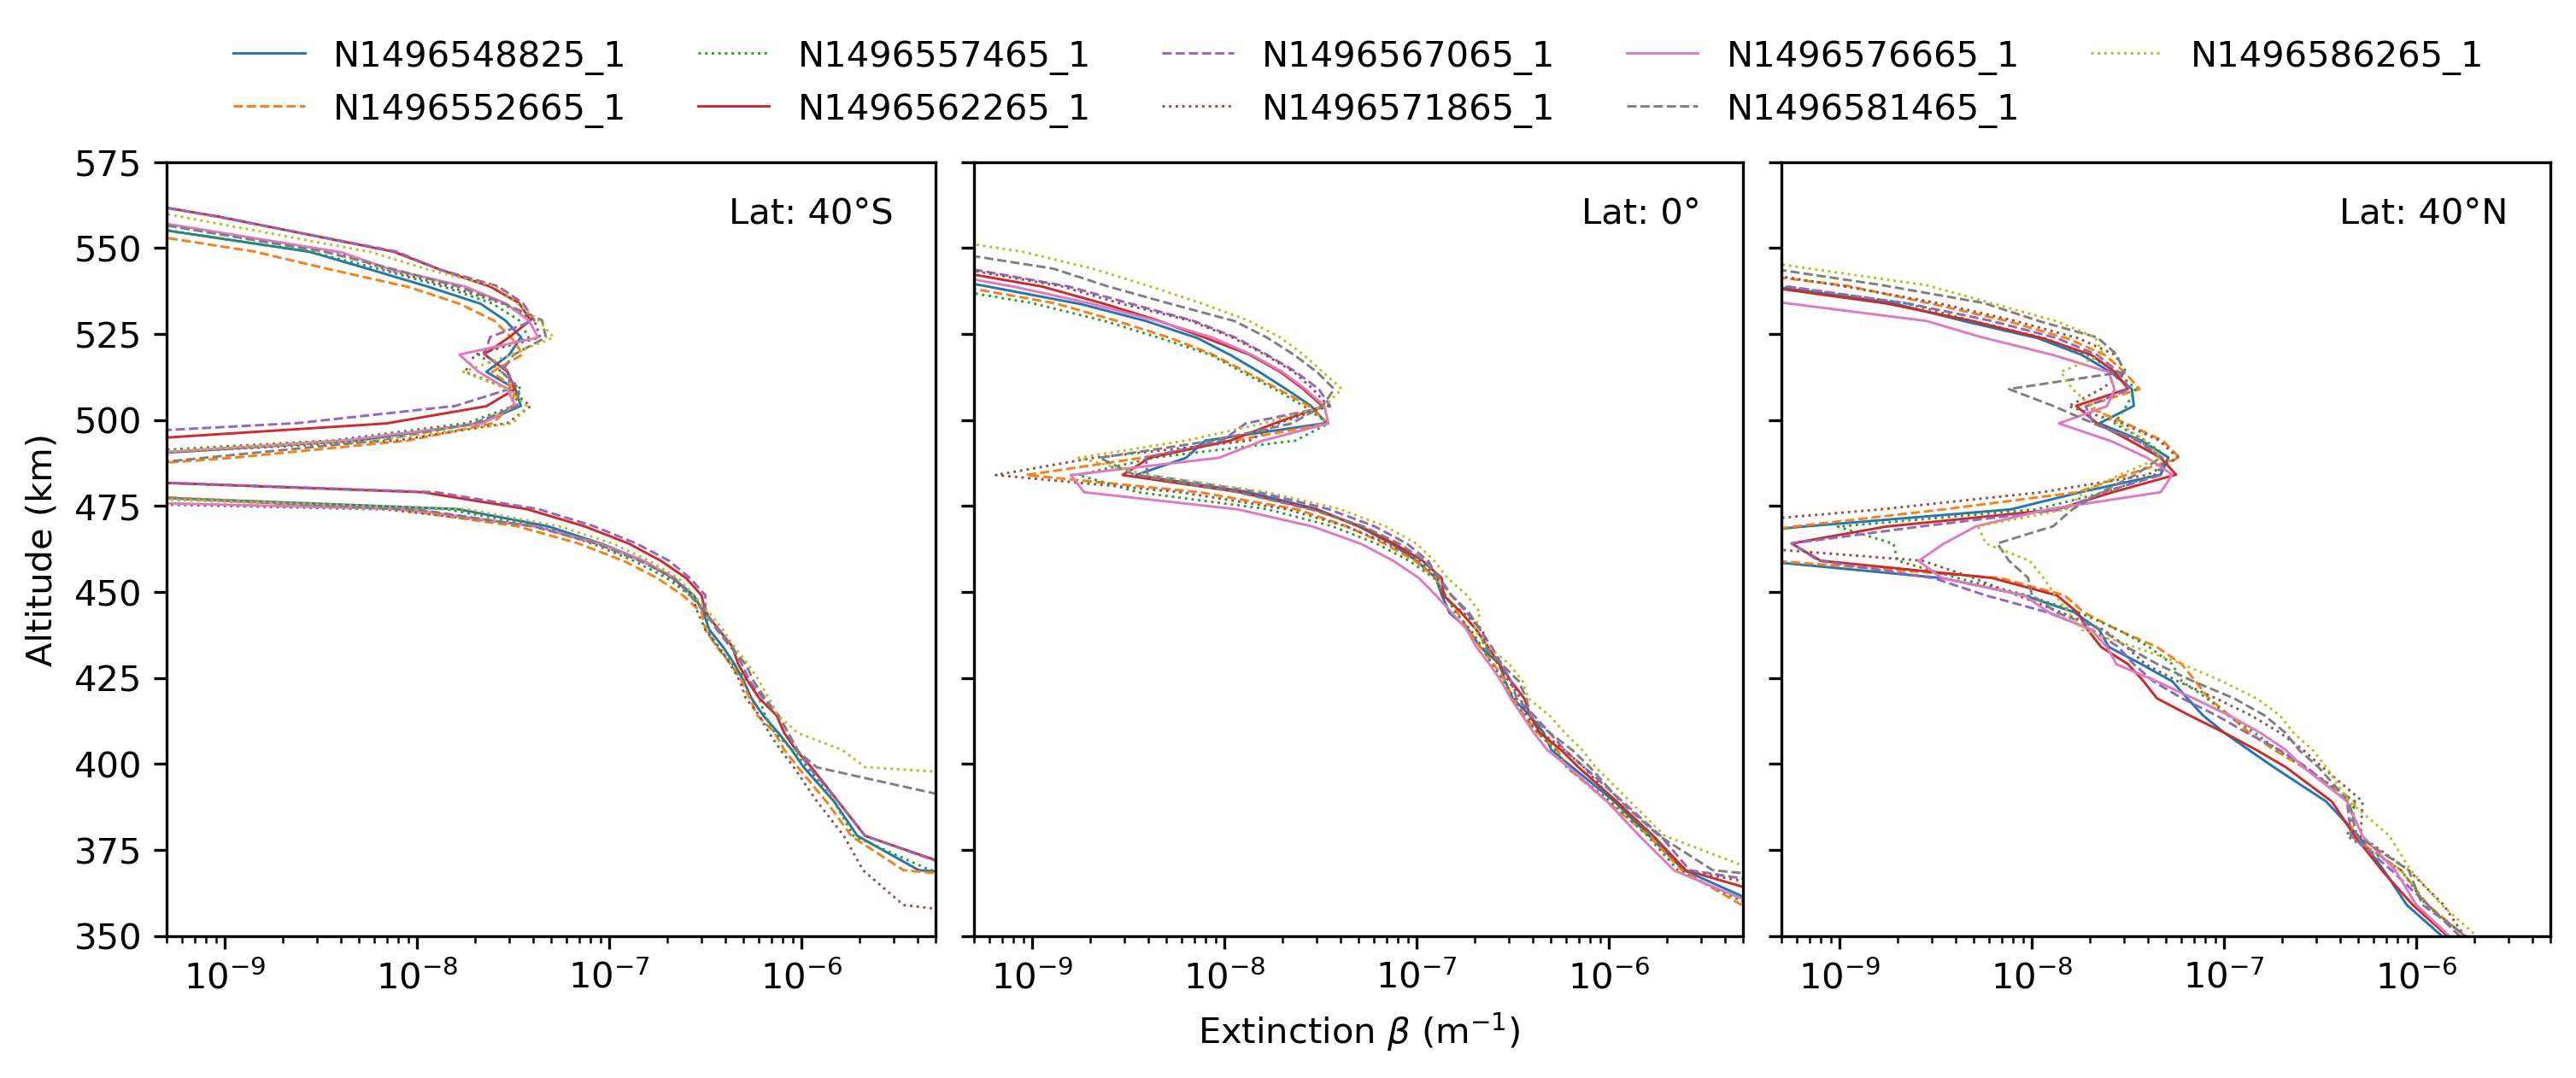
\includegraphics[width=\textwidth]{Fig/Time_variability.png}
    \caption{Extinction profiles for the series
    of 9 images taken 80 minutes apart in June 2005 (cf. Table \ref{tab:time_variability}).
    The global latitudinal map is shown in figure~\ref{fig:dhl_2004_2008}c.}
    \label{fig:time_variability}
\end{figure}

The figure~\ref{fig:time_variability} presents extinction profiles extracted from the analysis of these 9 images.
First, we confirm that our calibration method is reliable from one picture to the other and the overall
variability of the detached haze is very small. We clearly observe the double layering at \ang{40}S and \ang{40}N reported
previously. All the locations of the maximum of the extinction peaks are located within a small altitude range (smaller
than the 8 km of the pixel scale). Then, the vertical offsets which are observed at different times are consistent
with  the accuracy of the image navigation, and therefore are not significant. At the equator and at \ang{40}S, the detached
haze layer is well detached for all the profiles. When the vertical offset is accounter for, all the extinctions are found
with relative differences of about $\pm$ 10\% compared to the average value, except in the depletion zone between
the main and detached haze layers where difference can reach an order of magnitude (at \ang{0}) to several order of magnitude
(\ang{40}N). The variations outside the depletion zone are not significant. We note that the different behavior of the
N1496576665\_1 profile at \ang{40}S and below 450 km, compared to other profiles, is an artefact due to the inversion
process.

The variability in the depletion zone at the equator is probably due to the retrieval uncertainties. The differences in
extinction are about one order of magnitude, consistent with uncertainties between the two layers
\citep[\emph{e.g.}][]{West2018}, and without specific temporal evolution.
The variability observed at \ang{40}N, in the depletion zone around 460 km are significant for two reasons.
First, the differences are much larger than the expected uncertainty in this zone. Second, the sequence shows
a gradual and consistent increase of extinction with time. If these differences were due to uncertainties in
the retrieval procedure, it would have rather given a chaotic evolution of the extinction with time.

We also remark that the corresponding extinction map (Fig.~\ref{fig:dhl_2004_2008}c) shows that in the south,
the detached haze is well separated from the main haze by a well defined depletion zone. In the north, the depletion
zone is less well defined and the detached haze and the main haze are connected vertically by a residual haze.
The variation of this residual haze is the one reported in Fig.~\ref{fig:time_variability} at \ang{40}N.
We can not strictly determine if we are witnessing time or a spatial variations since both the time and the longitude
of the observations change simultaneously during the image sequence. We note that a rotation of \ang{5} in longitude
corresponds to a maximum shift of 250 km in distance (one tenth of Titan radius), possibly consistent with a spatial
variation of the haze extinction.

\subsection{Dawn and dusk sides}

Aside from short time and local variations, we also are interested in images showing simultaneously the two sides
of Titan. At low phase angle, the viewing geometry allows us to retrieve the haze extinction with both the
illuminated and the dark side of Titan simultaneously  (Fig.~\ref{fig:dawn_dusk}).
In this case, we can compare the dawn and dusk limbs for
specific latitudes. Although Titan's day is about 16 terrestrial
days, the time spent by the haze on the night side or dayside is much shorter.
First, the atmosphere is superrotating and at altitude around 400 or 500 km the zonal wind is comparable to or
larger than the rotation speed at the ground \citep{Flasar2005, Achterberg2011, Lebonnois2012, Lellouch2019}.
This makes the actual diurnal cycle for the high altitude hazes shorter than 16 days by a factor of 2 or more.
Secondly, at high altitude, sunlight penetrating beyond the geometric terminator further shortens the time spent in darkness.
Thus, effects on the haze should be produced by processes with timescales
comparable with a terrestrial day.

\begin{figure}[!ht]
    \centering
    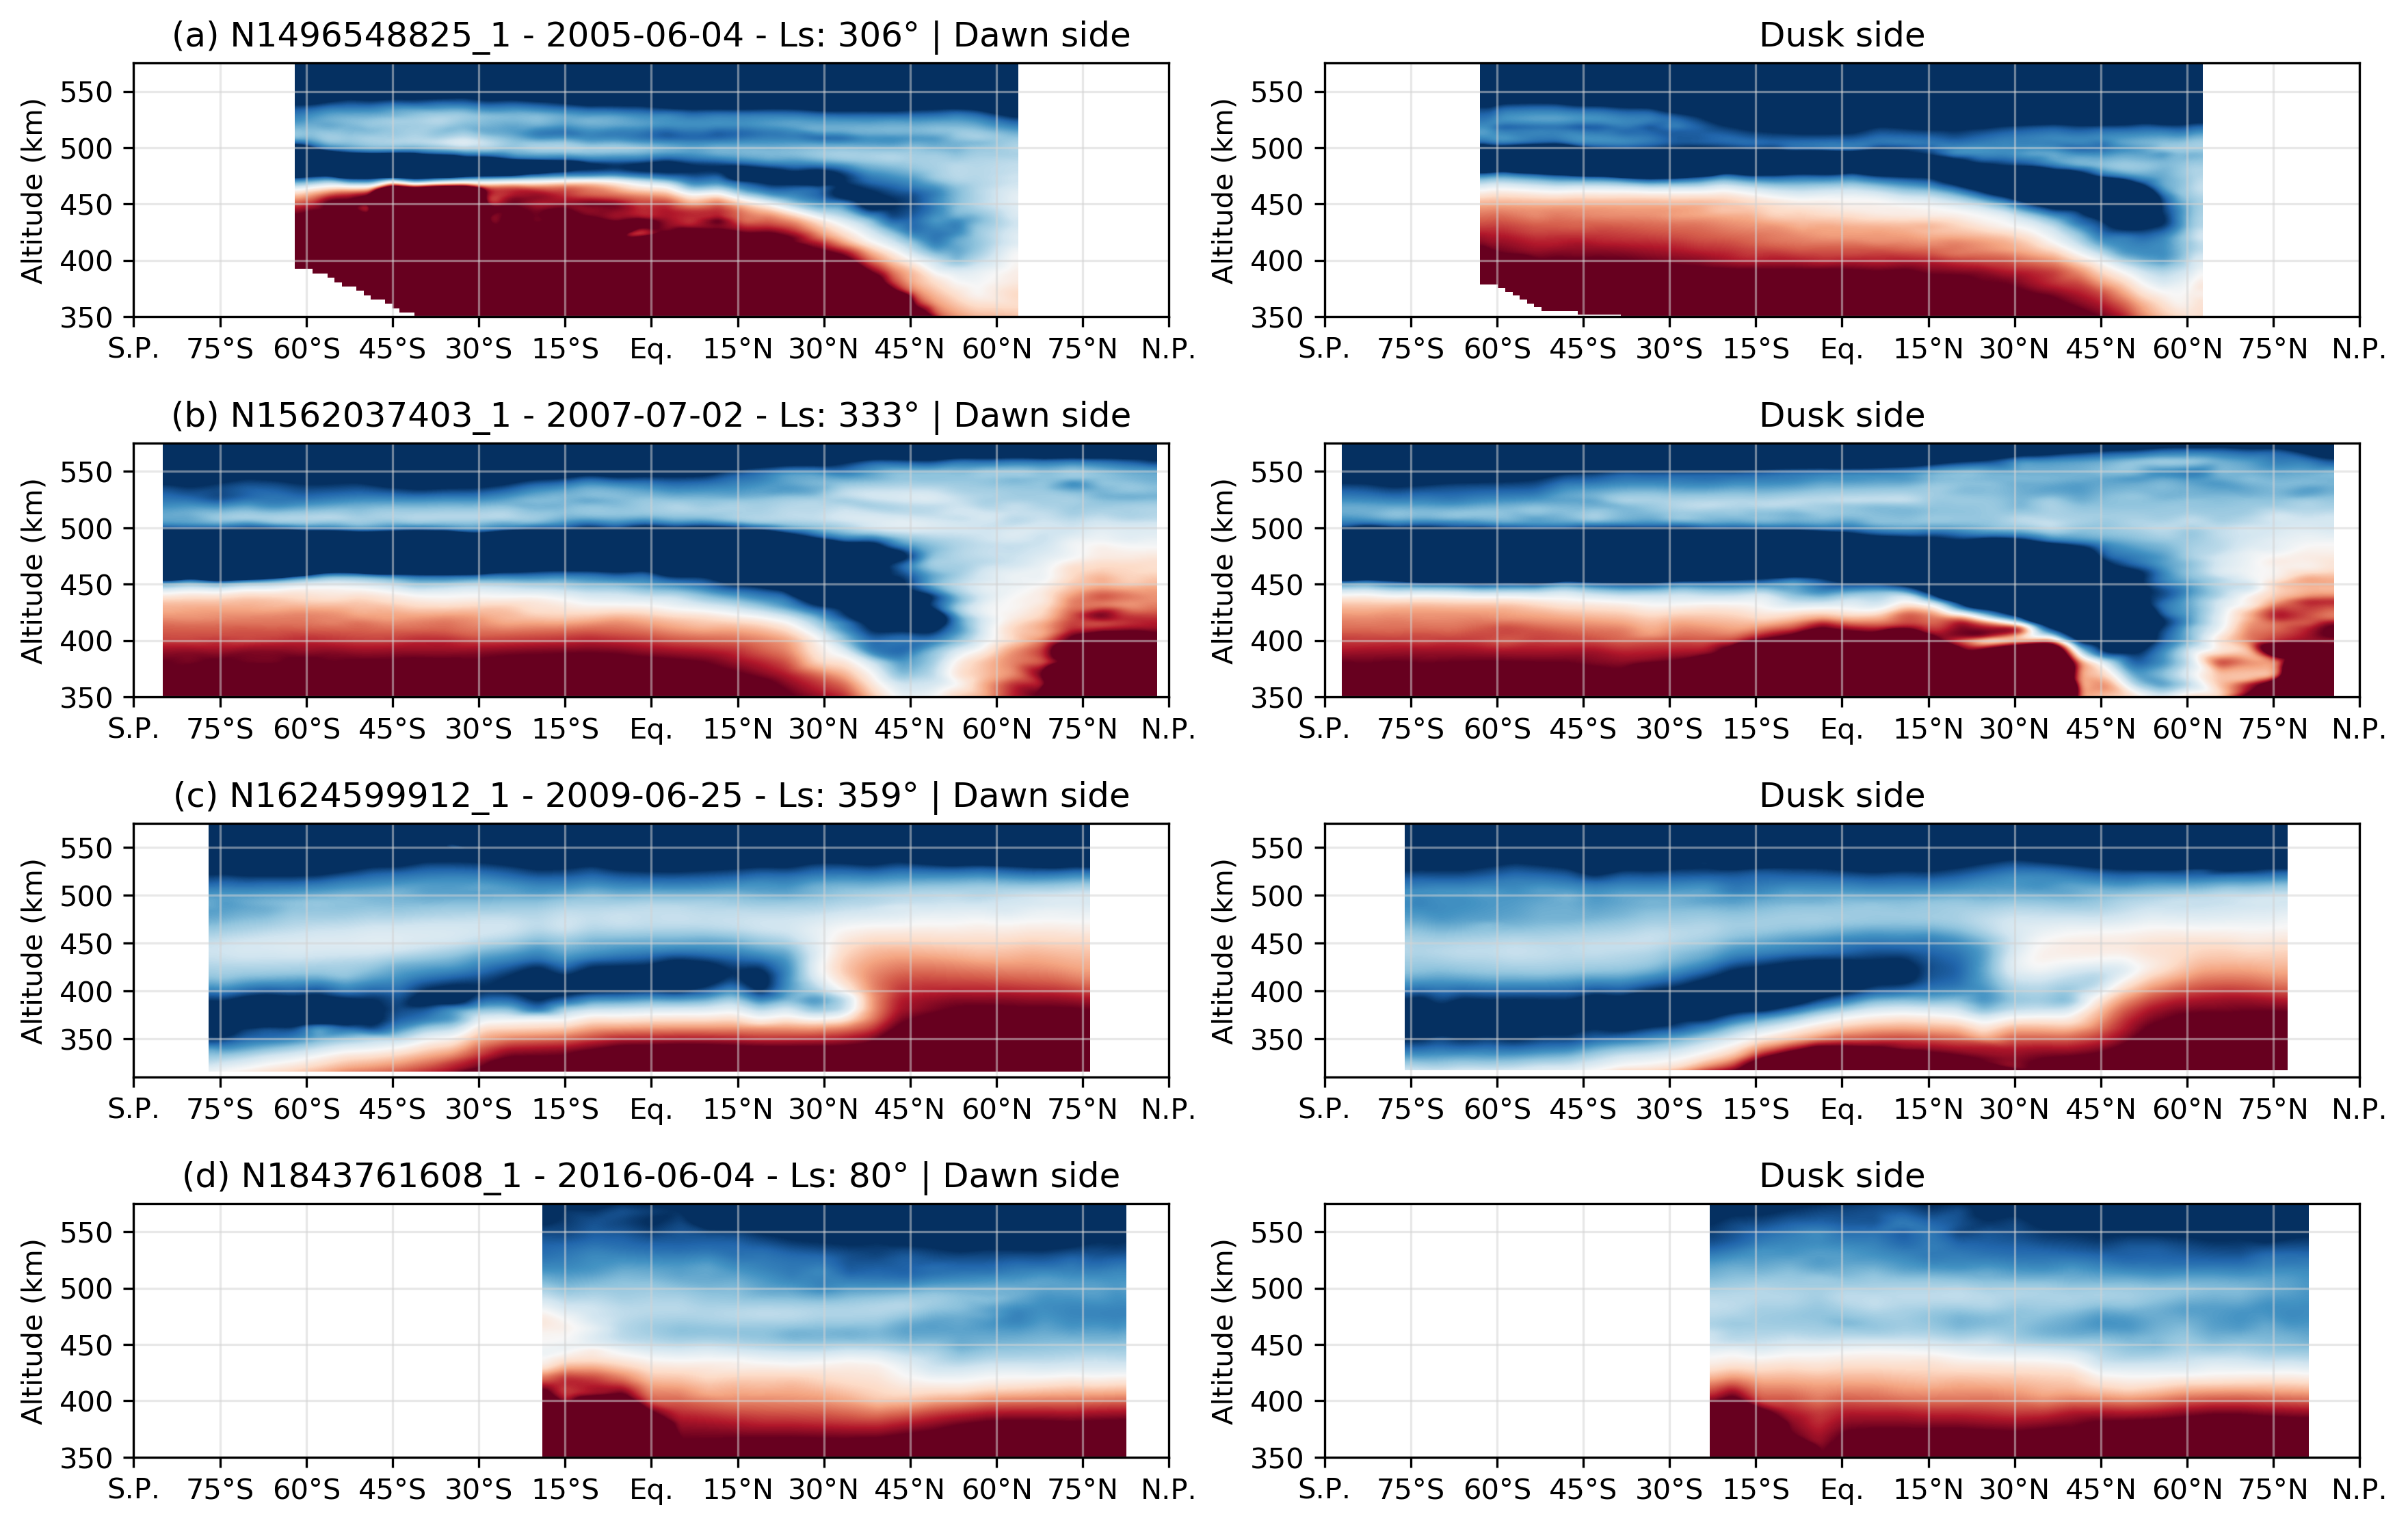
\includegraphics[width=\textwidth]{Fig/Dawn_dusk.png}
    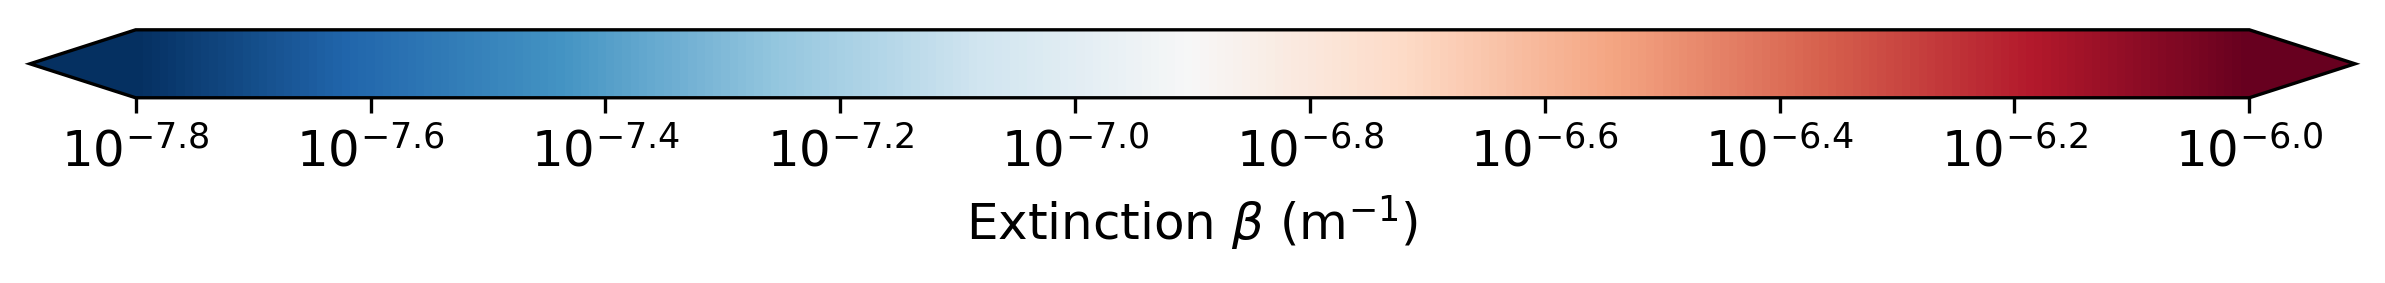
\includegraphics[width=.5\textwidth]{Fig/Extinction_colorbar.png}\vspace{-.3cm}
    \caption{The left and right panels show maps of the haze extinction for the dawn and dusk side of
    Titan for 4 different images taken during the mission when the viewing geometry allows us to observe both dawn and dusk
    limbs. The date and the seasonal solar longitude are provided for each image.}
    \label{fig:dawn_dusk}
\end{figure}

Figure~\ref{fig:dawn_dusk}a presents the haze extinction at the dawn and dusk sides as observed
in June of 2005 (Fig.~\ref{fig:dhl_2004_2008}c). The detached haze differs significantly between the two sides.
At the equator, we observe on the dawn side a double detached layer of 40 km thickness whereas it appears
as a thin layer of 10 km thickness on the dusk side. The haze extinction at the peak differs significantly,
from 7$\times 10^{-8}$ to 2.5$\times 10^{-8}$ m$^{-1}$, respectively. The depletion below the haze layer
is also less pronounced on the dawn side compared to the dusk side. Although this observation was taken
during the period of stability for the detached haze, we observed a significant asymmetry between
the dawn and dusk side. This asymmetry is also observed in all the images taken at the same moment which were
analyzed in section 4.1.

Two years later, another low phase angle image was recorded (Fig.~\ref{fig:dawn_dusk}b).
This time, the detached haze layer is much more symmetrical between the two sides. The peaks of haze extinction
are at the same altitude with comparable values. However, small differences can be noticed: there is a
small secondary layer above the detached haze layer at the dusk side between \ang{50}S and \ang{20}N, and may even extend 
northward. In the northern hemisphere, the extinction appears slightly larger at dawn that at dusk, and the
vertical extent of the detached haze is also a bit larger. However, the overall morphologies are very similar.

At the equinox, the detached haze layer already started its drop in altitude (Fig.~\ref{fig:dawn_dusk}c).
There are significant differences between the two sides, in both hemispheres, while at the equator the two
profiles are almost identical. The haze layer is not exactly symmetrical in the southern hemisphere. The detached
haze itself is at the same altitude, but the depletion zone is at higher altitude at the dawn side, and the main
haze layer is thinner in the dusk side. In the northern hemisphere, the haze layer is more complex, and the
asymmetry is even more marked with a detached haze at different altitudes and with a different extinction. The
detached and main haze layers at the dawn side appear optically thicker than the layers at the dusk side.
This is consistent with the two previous cases.

After the equinox, fewer images were taken at low phase angle. Among them, we do not notice any
significant differences between the dawn and dusk sides. After the reappearance of the detached haze layer in
2016, we found only one image with the relevant geometry to see both sides of Titan illuminated at the same time
(Fig.~\ref{fig:dawn_dusk}d). In this case, we are close to the solstice and the sub-solar latitude is almost
at its maximal extent and does not allow us to probe the southern high latitudes near the terminator.
The main haze appears very symmetrical on both sides and almost identical
above \ang{45}N. The depletion can be followed continuously all around the North Pole. At latitudes lower than
\ang{45}N, the values of the haze extinction are similar but the altitudes of the extinction peak differ by
25 km. We also observe partial secondary detached layers in each side, but not at the same latitudes.

The haze extinction profile and the altitude of the detached haze layer can differ significantly between the dawn
and dusk sides. In general we notice a higher extinction in the dawn side than on the dusk side. This effect
could be due to a diurnal cycle.
\subsection{Longitudinal variability}

\change{Due to orbital constrains, most of our observations sampled only a small range of longitudes.
However, a few} observations of Titan taken from a near-polar point of view offer a unique way to study the evolution of
the detached haze with a large coverage in longitude and within a small range of latitudes. It allows us
first to check the homogeneity of the haze in longitude, and it also allows us to extend our previous
observations between the dawn/dusk sides with a local time coverage between 6:00 and 18:00.

\begin{figure}[!ht]
\plotone{Fig/Lon_variability}
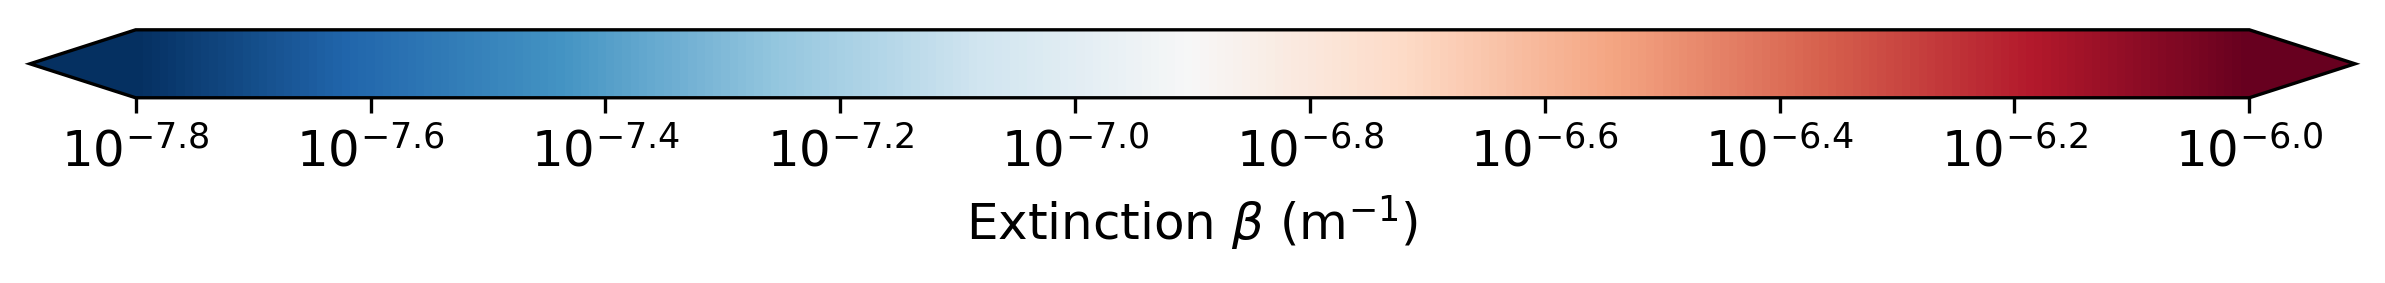
\includegraphics[width=.5\textwidth]{Fig/Extinction_colorbar}
\caption{The panels show the map of the haze extinction as a function of longitude and local
time for a set of 3 images taken in March and April, 2009 ($L_s=\ang{356}$). The latitude range covered is
also indicated for each image.}
\label{fig:lon_variability}
\end{figure}

We analyzed a set of three images taken sequentially within a month interval. The first observation
was performed on the 29$^{th}$ of March, 2009 (Fig.~\ref{fig:lon_variability}a) during the collapse of the detached
haze layer. Two other observations were made two weeks and one month later, with the same geometry
(Figs.~\ref{fig:lon_variability}b, \ref{fig:lon_variability}c). The detached haze layer is
located at 470 km at all the longitudes. Inside the depletion region, we notice a plume of haze
between 400 and 440 km and between \ang{150}W and \ang{220}W. In mid-April, the plume is located between
\ang{160}W and \ang{240}W and between 375 and 425 km. It appears disconnected and settling from the detached
layer, which remains at 470 km. At the end of April, we see the extension around 410 km and it
is spread from \ang{180}W and \ang{250}W. This aerosol plume is almost connected with the main haze.

This feature is not correlated with the local time but remains about at the same longitude and drifts slowly
toward the West. This would correspond to a retrograde motion of about 0.6 m/s. Another solution would be
prograde motion of 6.6 m/s, in phase with the sampling of 15 terrestrial days. The vertical speed, assuming
that the aerosol cloud dropped from 400 km to 375 km in one month would be $10^{-3}$ m/s. We also identified a
modulation in the extinction and in the geometrical thickness of both the detached haze layer and the main
haze. In the last image, only the geometrical thickness is modulated and not the haze extinction.

These observations show that the haze layer is not completely homogeneous in longitude and have some
fluctuations in extinction and in geometry.
It also strengthen the idea that space and time variations, as in observations previously discussed,
can not be distinguished without additional observations \change{(not available in this dataset)}.
The dawn/dusk differences and the short-term variations,
presented in the two previous subsections, could be due to longitudinal effect rather than to time variations.
Therefore, with the results of this section, we stress that the longitude inhomogeneities should be kept
in mind \change{as a secondary effect} when discussing and comparing latitudinal maps of the detached haze layer.
\section{Comparisons with UVIS occultations and GCM predictions}

\cite{West2018} already confirmed the excellent agreement between the observations made during
two Voyager flybys and the position of the detached haze layer one Titan year later.
Comparisons with Cassini Visual and Infrared Mapping Spectrometer (VIMS) and
Cassini Composite Infrared Spectrometer (CIRS) instruments, could be possible but
they are limited by the sensitivity of their detectors above 450 km where the detached haze is located.
Therefore, we only performed a comparison with two stellar occultations
made by the Cassini Ultraviolet Imaging Spectrograph (UVIS) instrument in 2009 \citep{Koskinen2011}.
The extinction profiles retrieved in the previous sections can also be compared with results
obtained with other instruments and with Global Circulation Model (GCM) predictions.

\subsection{Comparison with UVIS occultations}

\cite{Koskinen2011} derived information on the mesosphere and thermosphere of Titan using UVIS stellar
occultations. The sensitivity to haze opacity of UVIS during a stellar occultation is much better than what ISS can achieve. However,
while ISS probes the light scattered by the detached haze layer, UVIS probes the light transmitted through a tangential
path at the limb. In both cases, an extinction profile can be retrieved. ISS can retrieve the extinction of the
particles which scatter light, and under assumptions concerning the phase function and the single scattering albedo \change{\citep{Seignovert2017, West2018}}.
On the other hand, UVIS is able to retrieve the total extinction from transmission with no assumption about the haze
particles. This difference is valuable because it may give information about the change in aerosol
size with altitude. In practice, ISS sensitivity is not sufficiently sensitive to probe above
the peak of the detached haze by more than a scale height.

Two of the UVIS occultation profiles, in 2008 and 2009 (T41 and T53 flybys), can be directly compared with ISS
observations at the same location and at the same period (Fig.~\ref{fig:uvis_iss}). The UVIS profiles are scaled to
offset the spectral dependence between ISS and UVIS effective wavelengths (338 nm and 1850-1900~\AA~respectively).
This offset is due to the spectral dependence of the extinction cross-sections and to the intrinsic
differences arising from comparing the extinction retrieved from scattering properties or from occultation
\citep[see.][]{Cours2011}.

\begin{figure}[!ht]
\plotone{Fig/UVIS_ISS}
\caption{Comparisons between ISS and UVIS extinction profiles before the equinox.
UVIS profiles are retrieved by \cite{Koskinen2011} during the T41 (2008/02/23) and T53 (2009/04/19) flybys.
ISS profiles are retrieved for the images N1585329510\_1 (2008/03/27) and
N1618568958\_1 (2009/04/16).
The UVIS profiles are scaled by a factor 0.15 to compensate the spectral dependence of the extinction
cross section and overlap ISS retrievals.}
\label{fig:uvis_iss}
\end{figure}

\change{The two profile can be compare in the 450 to 550 km altitude range.
In the first case (Fig.~\ref{fig:uvis_iss}a), even if the profiles don't exactly overlaps, the ISS extinction profile presents a peak of extinction exactly at the same location as the one observed by UVIS. The drop, above and below the peak is more pronounced with ISS than with UVIS.
In the second case (Fig.~\ref{fig:uvis_iss}b), the two profiles presents a excellent agreement with each over in the 450 to 550 km altitude range.}

Considering that UVIS and ISS profiles are not taken simultaneously and
they don't probe the same longitude, the results of the previous section demonstrate that these differences are
consistent with the natural variabilities observed in the detached haze layer.
This comparison is then a good validation of our results concerning the extinction profiles of the detached haze.

Above 575 km, UVIS extinction profiles show the presence of a secondary layer at 610 km which is not detected
by ISS. As shown by \cite{Cours2011}, ISS is only sensitive to the larger aerosols, those that scatter light, whereas
UVIS is able to probe the extinction of all the particles, and especially the smaller ones which do not scatter.
In theory, the difference between UVIS and ISS above 575 km may reveal a sharp change in aerosol size distribution.
But, this layer is located at altitudes where the signal to noise is low and \change{our model is no longer able to retrieve the extinction above this altitude.}
Therefore, it is not possible to draw a safe conclusion from the ISS profiles above 575 km.

\subsection{Comparison with general circulation models predictions}

General circulation models are very powerful tools to understand the climate of planetary atmospheres and the
interplay between different processes at planetary scale. In the case of Titan, circulation and haze are linked
by a strong feedback loop. The large scale structures in the haze layer are produced by the action of the
circulation. The haze layer produces a feedback effect on the circulation through the control of the stratospheric
thermal structure \citep{Rannou2004}. The detached haze is one of the noticeable feature produced by the the
stratospheric circulation \citep{Rannou2002, Lebonnois2012, Larson2015}. The figure.~\ref{fig:gcm_winter}
and \ref{fig:gcm_spring} show the maps of haze extinction obtained by \cite{Lebonnois2012} and
\cite{Larson2015} at 700 nm and 525 nm respectively. They can be compared with the extinction map derived
with ISS in the CL1-UV3 filters at 338 nm.

\begin{figure}[!ht]
    \centering
    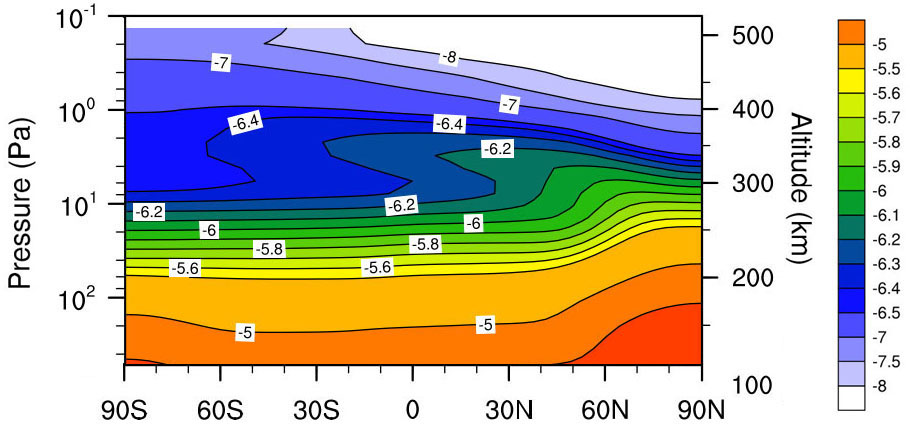
\includegraphics[width=.4\textwidth]{Fig/Lebonnois2012_Fig4_winter.jpg}
    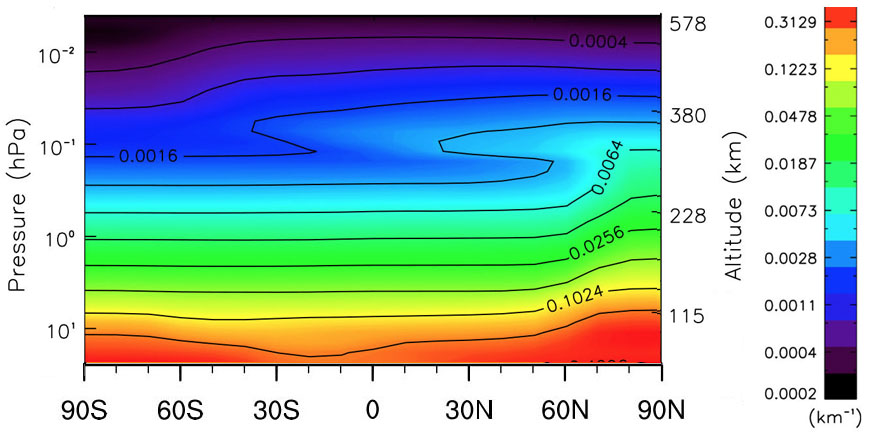
\includegraphics[width=.4\textwidth]{Fig/Larson2015-Fig7_Winter.jpg}
    \includegraphics[width=.8\textwidth]{Fig/N1477222048_2-lat_beta.png}
    \caption{At the top, the zonally averaged haze extinction at the northern winter solstice
        ($L_s = \ang{270}$) estimated by \cite{Lebonnois2012} at the wavelength $\lambda = $ 700 nm (left)
        and by \cite{Larson2015} at $\lambda = $ 525 nm (right). At the bottom, haze extinction map
        retrieved from Cassini/ISS observation CL1-UV3 ($\lambda = $ 338 nm) in the middle of the winter
        (\textbf{N1477222048\_2} - $L_s = \ang{300}$).}
    \label{fig:gcm_winter}
\end{figure}

At the northern winter solstice (Fig.~\ref{fig:gcm_winter}), the detached haze appears around 350 km
in both models. In \cite{Lebonnois2012}, the altitude decreases by about few tens of km from the southern latitudes to
the north polar region where it merges with the north polar hood at ($\simeq$ \ang{40}N). In \cite{Larson2015}, the detached
haze remains at constant altitude, appears better marked than in \cite{Lebonnois2012}, and merge with the polarhood
around \ang{60}N. In both models, the extinction increases from the south to the north by about a half magnitude.
In the observations made in 2004, \emph{i.e.} at the middle of the winter, the detached haze layer is completely developed at
500 km and covers latitudes from the south polar region to \ang{60}N where it merges with the north polarhood. The
location of the depletion zone decreases from 475 to 425 km between \ang{40}N and \ang{60}N, which is not the case in
models. It is, on the other hand, consistent with the results obtain from stellar occultation by \cite{Sicardy2006}.
The haze extinction increases from the south to the north with about the same magnitude than in models. This
is consistent with a layer increasing in aerosol loading while the airmass is flowing from south to north. It was already
noted \citep{West2011, West2018} that the detached haze layer in models appears as a supplementary layer added to
the background aerosols while, in data, it appears detached because there is an intermediated zone strongly depleted in
aerosols. Finally, as mentioned before, the detached haze layer is continuous all around the South Pole, which is not
the case in the models.

\begin{figure}[!ht]
    \centering
    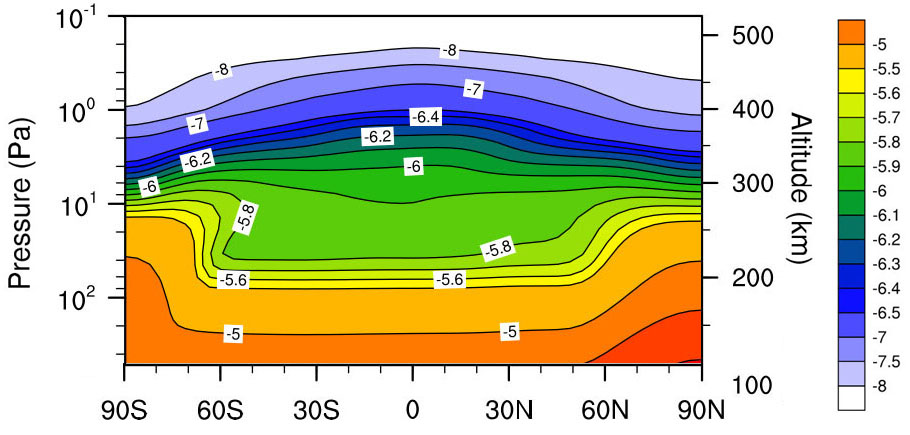
\includegraphics[width=.4\textwidth]{Fig/Lebonnois2012_Fig4_equinox.jpg}
    \includegraphics[width=.4\textwidth]{Fig/Larson2015-Fig7_Spring.jpg}
    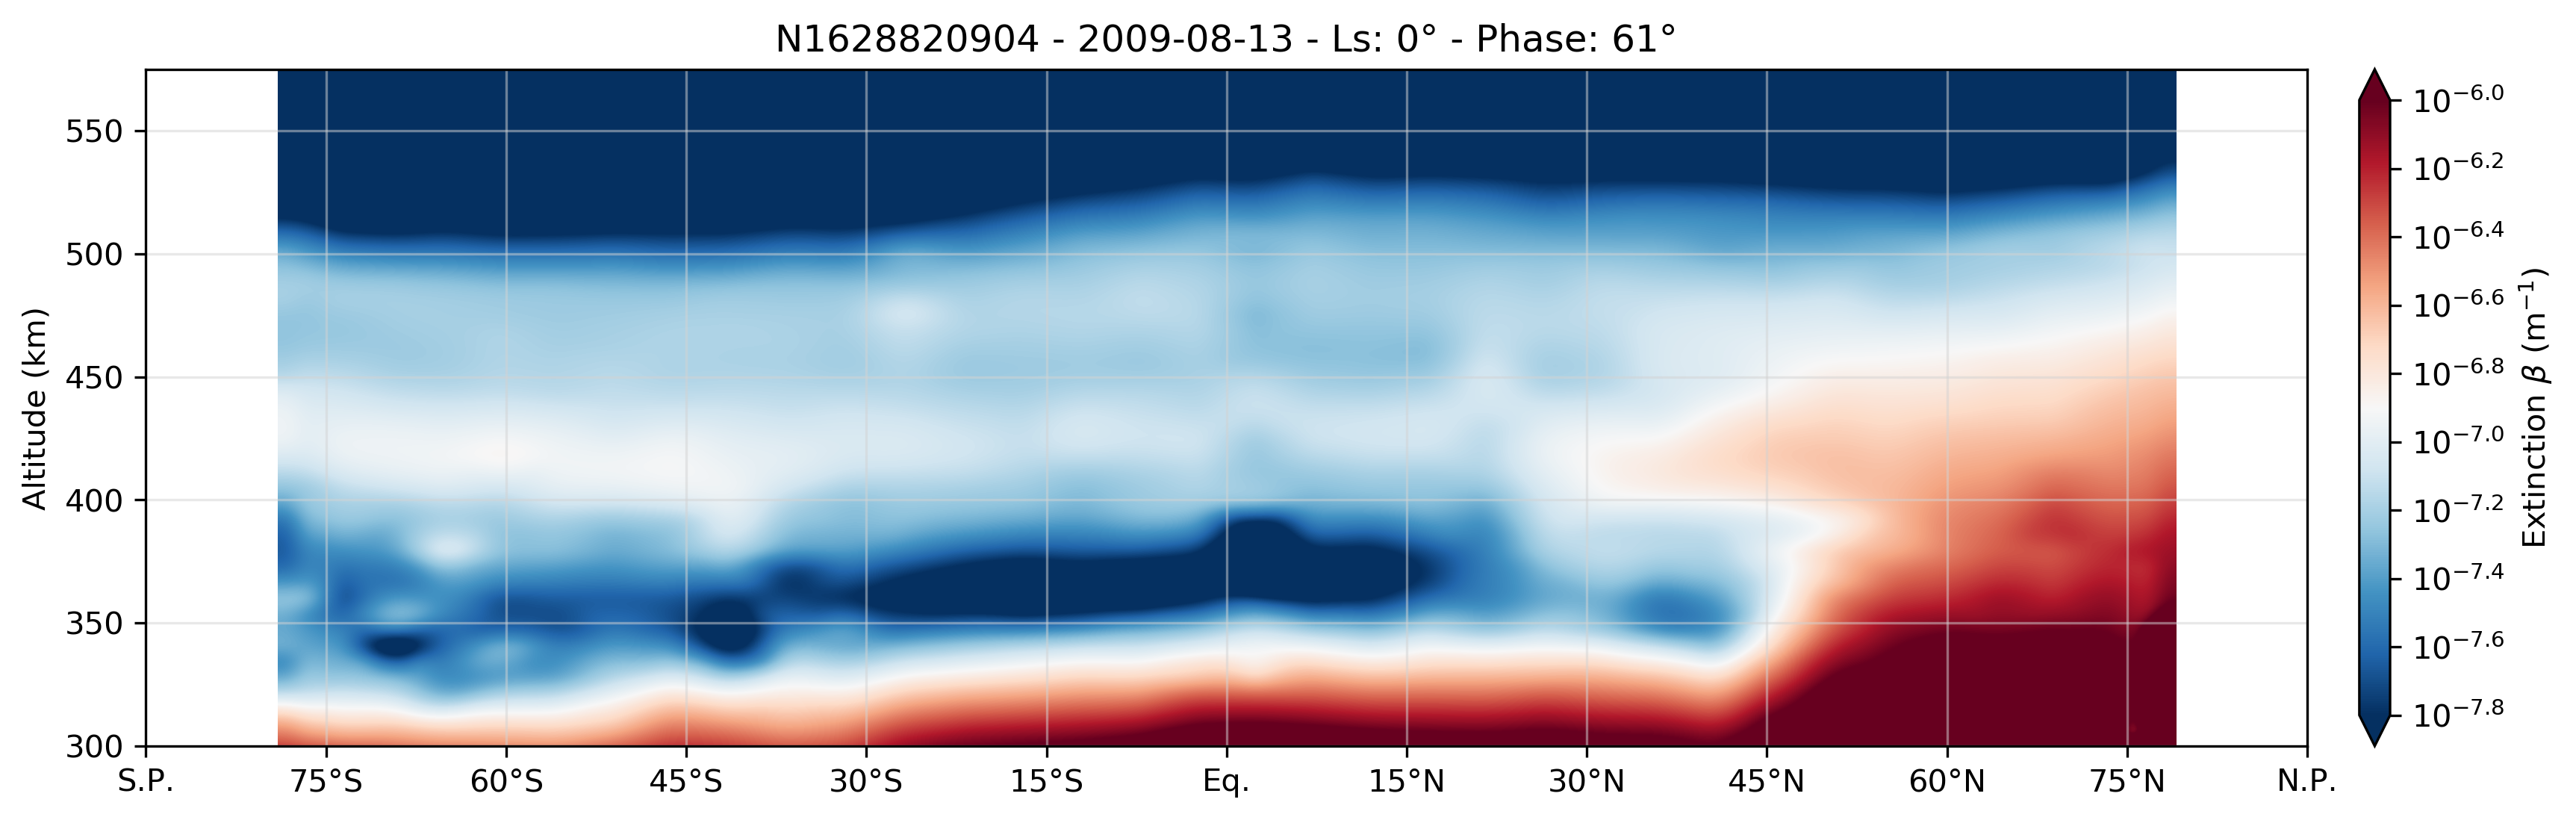
\includegraphics[width=.8\textwidth]{Fig/N1628820904_1-lat_beta.png}
    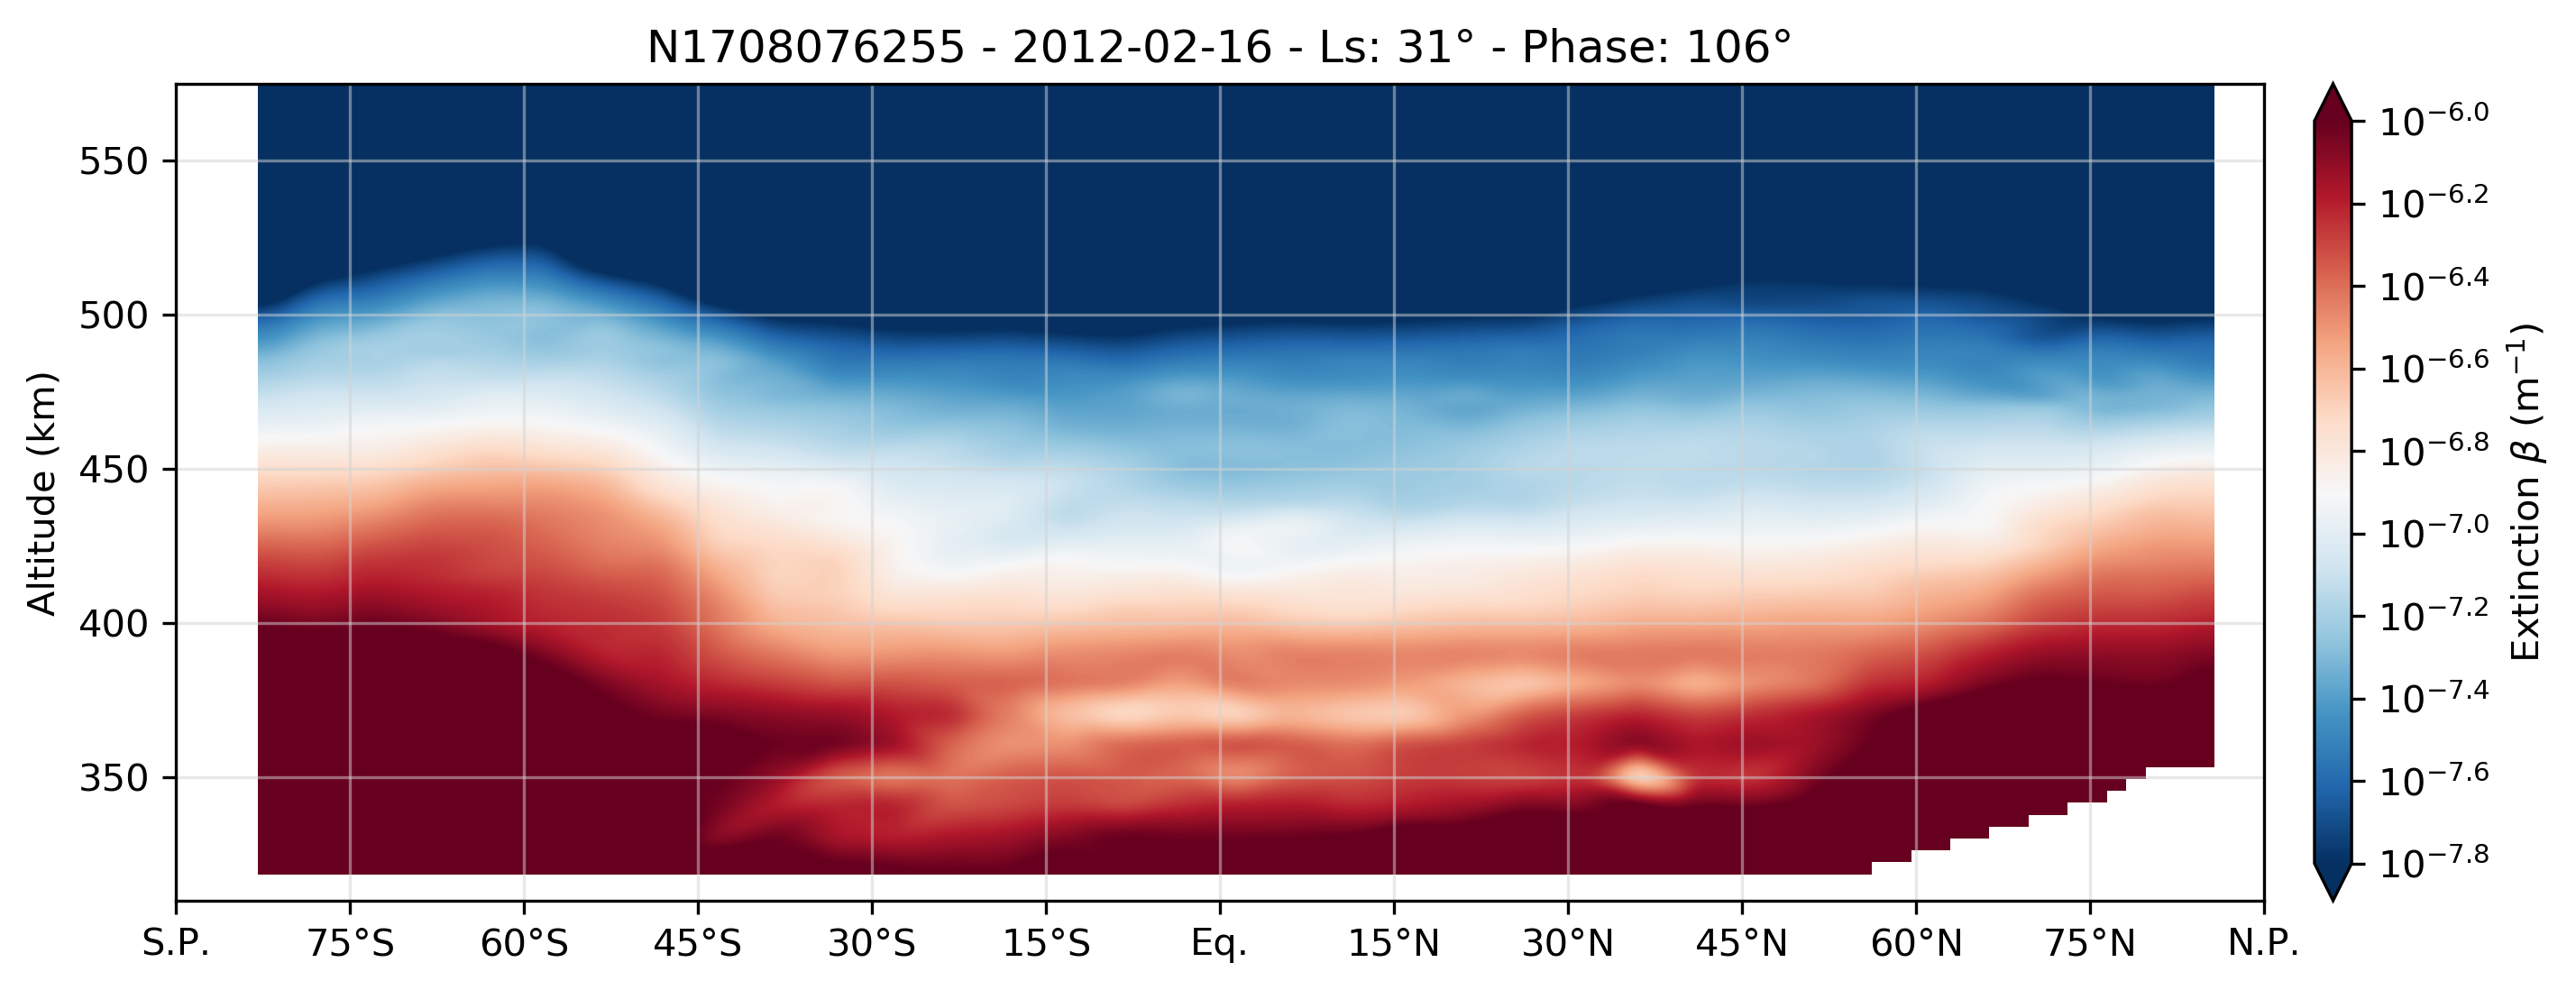
\includegraphics[width=.8\textwidth]{Fig/N1708076255_1-lat_beta.png}
    \caption{At the top, the zonally averaged haze extinction at the northern spring equinox ($L_s = \ang{3}$)
        estimated by \cite{Lebonnois2012} (left) and at 1000 days after the equinox ($L_s = \ang{30}$)
        by \cite{Larson2015} (right).
        At the bottom, two panels showing the haze extinction map retrieved from the Cassini/ISS observations
        at the Northern Spring equinox (\textbf{N1628820904\_1} - $L_s = \ang{0}$) and 1000 days after the equinox
        (\textbf{N1708076255\_1} - $L_s = \ang{30}$).}
    \label{fig:gcm_spring}
\end{figure}

At the northern spring equinox (Fig.~\ref{fig:gcm_spring}), the model from \cite{Lebonnois2012} shows a
flat main haze layer without detached haze between \ang{60}S and \ang{60}N and with two major increases at both poles. The
haze at south is increasing as a consequence of the circulation reversal while the northern haze is no more feeded
and will disappear later in the season. In observations (first panel of Fig.~\ref{fig:gcm_spring}),
this thicker haze is observed only for the northern latitudes, the detached haze has not yet disappeared and
and the feeding of the south polar haze has not started yet. To notice a major increase of extinction at the South Pole,
we need to wait until the beginning of the spring at $L_s = \ang{30}$ (second panel Fig.~\ref{fig:gcm_spring}).
At that period, the detached haze layer almost completely collapsed on the main haze and the haze distribution is very
similar to the one predicted by \cite{Lebonnois2012} at the equinox. In \cite{Larson2015}, 1000 days after the equinox,
we also observed a \emph{U} shape in the haze extinction as in data, but in this case, a new detached haze layer already
started to grow from the South Pole in the model whereas in data (second panel  of Fig.~\ref{fig:gcm_spring}) the local
increase seen at 380 km is the consequence of the drop of a previous secondary layer (cf. Figs.~\ref{fig:dhl_2008_2012}g
and \ref{fig:dhl_2008_2012}h). In both comparisons, this means that the timing in the circulation models is not in
phase with the reality. The model of \cite{Lebonnois2012} seems to be in advance by about 3 years compared to the data.
We have not enough information to characterize the advance in phase of \cite{Larson2015} model.

The timing and the scale of the drop predicted by both models (Fig.~\ref{fig:gcm_cycle}) globally match
the observations after the vernal equinox. The abrupt decrease of the vertical winds could be the cause of the fall of
the detached haze layer at the aerosol terminal speed. On the other hand, the timing and the scale of the reappearance
of the detached haze layer in models does not follow exactly the observations. Announced in late 2014 or early 2015
($L_s = \ang{60}$) by \cite{Larson2015} or in mid-2017 ($L_s = \ang{90}$) by \cite{Lebonnois2012}, the detached haze layer
finally reappeared in late 2015 to early 2016.
However, in May 2017, the upper atmosphere of Titan is still evolving and does not present a polar hood in the South Pole
similar to the one observed in 2004. Moreover, the most recent observations of mid-2017 seem to show that the seasonal
formation of the detached haze layer could be different from one hemisphere to the other. The double peaks at
420 and 450 km in the temperature gradient profile, a proxy for the haze extinction, obtained from the 1989
occultation \citep{Sicardy1999} supports this hypothesis.

\begin{figure}[!ht]
    \centering
    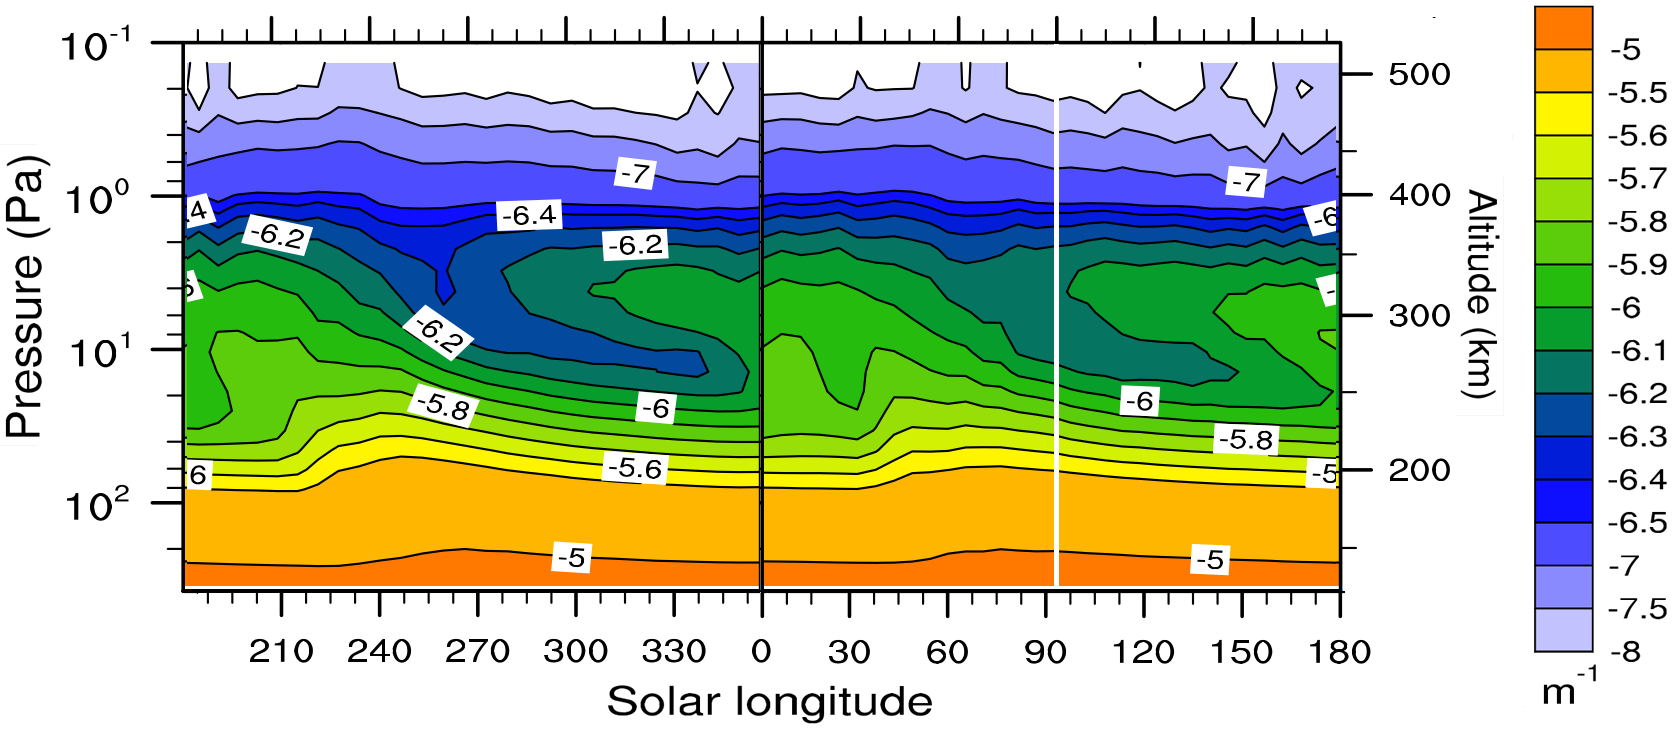
\includegraphics[width=.4\textwidth]{Fig/Lebonnois2012_dhl_cycle.png}
    \includegraphics[width=.4\textwidth]{Fig/Larson2015_dhl_cycle.png}
    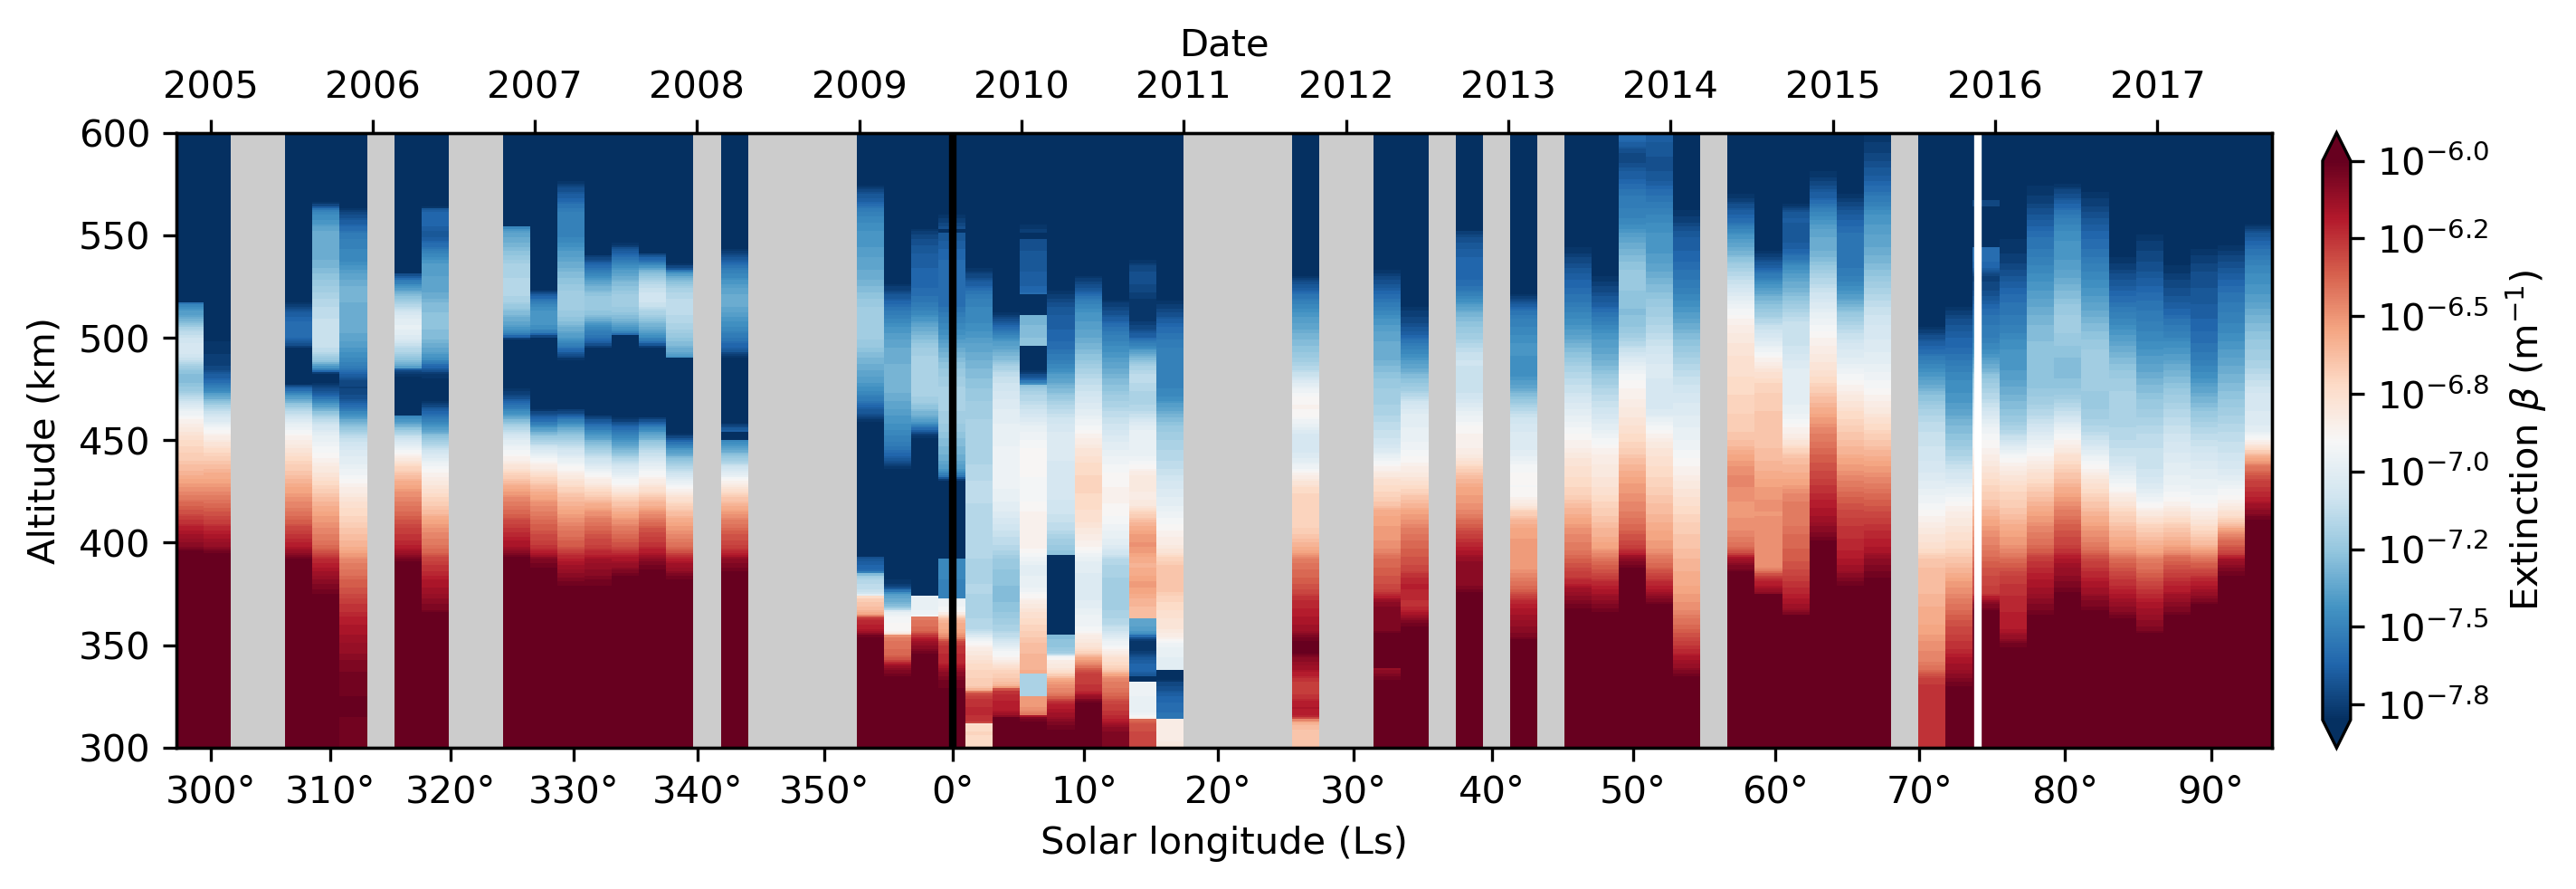
\includegraphics[width=.8\textwidth]{Fig/DHL_time_eq.jpg}
    \caption{Top-right: the annual variations of the zonally averaged equatorial opacity at 700 nm adapted
        from \cite{Lebonnois2012}.
        Top-left: the seasonal evolution of the aerosols mass density (g/cm$^3$) adapted from \cite{Larson2015}. The white dots are the local maximum of extinction extracted from the model.
        In both figures, the white vertical line correspond to the predicted date of the reappearance of the
        detached haze layer (after $L_s = \ang{90}$ and after $L_s = \ang{60}$ respectively).
        Bottom: the haze extinction as a function of time an altitude at the equatorial.
        % FIXME: Redo alt vs. time plot at Eq.
    }
    \label{fig:gcm_cycle}
\end{figure}

The current general circulation models do not match some of the large scale features reported before. The first of them
is the shape of the vertical extinction profile which has a local depletion, producing the detached haze layer, in the
observations while it simply appears as a high altitude haze layer superimposed to the main background haze in models.
The amplitude of the observed depletion reported, before and during the collapse, is sufficient to consider that the
detached haze layer is really disconnected from the main haze. We already stressed that the detached haze layer is
continuous around the South Pole without any visible upwelling coming from the main haze at this location. Finally, we
reported an early contraction of the main haze in 2008, just before the drop of the detached haze at the equinox. The origin
for such a contraction should be related with the weakening of the Hadley cell when the latitudinal illumination gradient
decreases around the equinox.

Thanks to high spatial resolution of the ISS NAC camera, we noticed some small scale structures which could be unresolved or
erased by the temporal averaging in GCMs. During the northern winter and spring, we observed some sporadic decreases and
bursts in the extinction profiles at very short time scale. These events could have a major impact on the redistribution of
aerosols in the upper atmosphere. We also reported in numerous cases, the existence of sub-layers above the main detached
haze with large latitude extend. Usually, their presence could be followed during more than an Earth year. This is
especially true during the collapse of the main detached haze layer after the equinox, when we observed several smaller
drops from 500 km down to 300 km. And finally, the double structure reported in 2016-2017
(Figs.~\ref{fig:dhl_2015_2017}c and \ref{fig:dhl_2015_2017}d) with two very distinct detached haze layers in the
North at 450 km, in the South at 520 km, was never mentioned before and needs a new interpretation.

\section{Conclusions}

In this article we have analyzed observations of light scattered at the limb of Titan with ISS (UV3 filter) on the
Cassini spacecraft. We retrieved the haze extinction as a function of altitude, latitude and time between October 2004 and
September 2017. We followed, during about half Titan's year, the evolution of the DHL and the top of the
main haze. In particular, we witnessed the collapse of the DHL during the equinoctial transition of the atmospheric
circulation and its reappearance before the following solstice.

We confirmed and gave details about the collapse of the detached haze layer previously reported by \cite{West2011}.
We also tracked the small-scale variations after the equinox in order to detect the reappearance of the detached haze
layer at the end of 2015 \citep{West2018}. These two previous works focused on the DHL at equator. Here, we give
a full description of the structures of the haze layer as a function of altitude, latitude and time. We find
that the DHL has a natural variability, which can be temporal and spatial, and sometimes two distinct hazes or plumes
can be observed above the DHL. The amount of data is not large enough to distinguish between spatial or
longitudinal variability. But data taken with a polar viewing indicates that the haze is not completely
uniform in longitude.

The equinoctial collapse starts in the summer hemisphere. Its initial phase can be discerned in March, 2008.
The main haze collapses first and then the detached haze layer about one terrestrial year later. By April, 2012,
the detached haze is below 300 km and can not be seen at UV wavelengths.
The fall of the detached haze layer between 2009 and 2011 occurred at the average speed of -67 km/yr.
During the equinoctial collapse, the DHL seems to settle down at the aerosol terminal speed,
as reported by \cite{West2018}. If sedimentation does control the speed of the collapse,
it would indicate an absence of vertical wind at these two moments.
During a period of 3 years and a half (from mid-2011 to 2015), no stable detached haze layer was observed.
However, the haze layer fluctuates, and sporadic local detached layers appeared and disappeared rapidly.

The detached haze layer reappeared in December 2015. We first noticed this new detached haze when it was marginally
apparent in UV3 images.
The timing of the reappearance is offset compare to GCM predictions and it occurs with patterns more complex
that those predicted. First, it reappeared around 500 km in December, 2015 ($L_s =\ang{74}$) as a very faint
structure which became persistent and more pronounced with time.
At the equator this structure sedimented and finally disappeared in about one year, whereas it remained visible in the northern hemisphere.
A second detached haze appeared in July, 2016 around 500 km altitude, above the first DHL, and apparently started to settle down
as well. Unfortunately, the survey was interrupted in September 2017 by the end of Cassini mission. This second detached
haze layer did not cover all latitudes, was quite variable, and was present up to the final observation.

Unfortunately, no data were acquired between April 2008 and February 2009 and between December 2010 and September 2011.
We thought to use the NAC UV1 and UV2 images but these data have a very poor signal to noise ratio and
can not be included in our analysis.
However, a few images are available with the WAC camera in the VIO (Violet), BL1 (Blue) filters.
The behavior of the aerosols at these wavelength should be very similar to the UV3 filter and could fill these gaps.
It would also be interesting to perform similar analysis with data acquired through filters at larger wavelengths.
In these case, it would be possible to probe deeper layers in order to monitor the collapse of the DHL further
down and, as well, the cycle of the main haze. For instance, \cite{Rages1983} could probe as lower as 200-250 km
in clear filter ($\lambda_{eff} \simeq 0.5 \mu$m). At even longer wavelengths, we could reach levels in the low
stratosphere and, maybe probe high altitude polar clouds \citep{deKok2014,West2016}.

Comparison with General Circulation Models are fruitful. Our results reinforce, the scenario of a
detached haze cycle primarily controlled by circulation as proposed by \cite{Toon1992} with a 1D model, \cite{Rannou2002}
with a coupled 2D-GCM and \cite{Lebonnois2012, Larson2015} with coupled 3D-GCMs. Although GCMs capture the global
haze cycle, many differences remain, mainly driven by technical limitations.
\section*{Acknowledgments}

This work was supported by the French ministry of public research. The authors also thank the Programme National de Plan\'{e}tologie (PNP) for their financial support.
B.S. and R.W. thanks the Cassini Mission. Part of this work was performed by the Jet Propulsion Laboratory, California Institute of Technology.
P.R. thanks the French Agence Nationale de la Recherche (ANR Project APOSTIC No. 11BS56002, France).
B.S. thanks the Planetary Rings Node (SETI Institute) for their excellent PDS \href{https://tools.pds-rings.seti.org/opus}{browser interface OPUS}.

\section*{Data availability}
All the ISS extinction profiles derived from this analysis and the source code to produce the figure will be made
publicly available after publication on the \href{https://data.caltech.edu}{Caltech Data Archive},
doi:\href{https://doi.org/10.22002/d1.xxxx}{10.22002/d1.xxxx}.

\bibliography{biblio}
\bibliographystyle{aasjournal}

\end{document}
